\documentclass[12pt,a4paper,twoside,titlepage]{book}

% inclusione librerie
% NB: il pacchetto hyperref va caricato per ultimo ma prima del pacchetto 
% glossaries altrimenti l'indice del PDF non viene generato correttamente!
\usepackage[italian]{babel}
\usepackage{tikz}
\usepackage{graphicx}
\usepackage{frontespizio}
\usepackage[Lenny]{fncychap}
\usepackage{longtable}
\usepackage{minted}
\usepackage{pgf-umlsd}
\usepackage[bookmarks]{hyperref}
\usepackage[acronyms]{glossaries}

% impostazione interlinea
\linespread{1.2}

% configurazione tikz
\usetikzlibrary{automata, positioning, arrows, shapes}
\tikzset{->, >=stealth', node distance=5cm, initial text=$ $}

% configurazione minted
\setminted{
    frame=lines,
    framesep=2mm,
    baselinestretch=1.2,
    fontsize=\footnotesize,
    linenos
}

% necessario per far funzionare il pacchetto per glossari/acronimi
\makeglossaries

% acronimi
\newacronym{iot}{IoT}{Internet of Things}
\newacronym{aws}{AWS}{Amazon Web Services}
\newacronym[\glslongpluralkey={Radiatori Elettrici}, \glsshortpluralkey=RE]{re}{RE}{Radiatore Elettrico}
\newacronym{gpio}{GPIO}{General Purpose Input Output}
\newacronym{adc}{ADC}{Analog to Digital Converter}
\newacronym{mcu}{MCU}{Micro Controller Unit}
\newacronym{uart}{UART}{Universal Asyncronous Receive and Transmit}
\newacronym{tls}{TLS}{Transport Layer Security}
\newacronym{usb}{USB}{Universal Serial Bus}
\newacronym{rf}{RF}{Radio Frequenza}
\newacronym{ota}{OTA}{Over The Air update}
\newacronym{hmi}{HMI}{Human Machine Interface}
\newacronym{ble}{BLE}{Bluetooth Low Energy}
\newacronym{http}{HTTP}{Hyper Text Transfer Protocol}
\newacronym{spi}{SPI}{Serial Peripherial Interface}
\newacronym{ci}{CI}{Continuos Integration}
\newacronym{cd}{CD}{Continuos Delivery}
\newacronym{vmc}{VMC}{Ventilazione Meccanica Controllata}
\newacronym{rgbw}{RGBW}{Red Green Blue White}
\newacronym{ntc}{NTC}{Negative Temperature Coefficient}
\newacronym{led}{LED}{Light Emitting Diode}
\newacronym{rtos}{RTOS}{Real Time Operating System}
\newacronym{rtc}{RTC}{Real Time Clock}
\newacronym{ap}{AP}{Access Point}
\newacronym{sta}{STA}{Station}
\newacronym{pwm}{PWM}{Pulse Width Modulation}
\newacronym{sdk}{SDK}{Software Development Kit}
\newacronym{yat}{YAT}{Yet Another Thermostat}
\newacronym{cu}{CU}{Connection Unit}
\newacronym{red}{RED}{Radio Equipment Device}
\newacronym{emc}{EMC}{Electro Magnetic Compliance}
\newacronym{bt}{BT}{Bassa Tensione}
\newacronym{sil}{SIL}{System Integrity Level}
\newacronym{ca}{CA}{Certification Authority}
\newacronym{json}{JSON}{JavaScript Object Notation}
\newacronym{sntp}{SNTP}{Simple Network Time Protocol}
\newacronym{ncm}{NCM}{Network Connection Manager}

% glossario
\newglossaryentry{mqtt}{
    name=MQTT,
    description={Protocollo di scambio di messaggi di tipo publish/subscribe pensato 
        per l'utilizzo su dispositivi con scarse risorse hardware, quali ad esempio 
        i dispositivi \acrshort{iot}}
}

\newglossaryentry{micro}{
    name=microcontrollore,
    description={Componente elettronico che integra in un unico chip processore, memoria
        RAM, memoria flash, gestione delle periferiche di input/output \acrshort{gpio}. Tipicamente offre 
        prestazioni molto limitate ma bassi costi e bassi consumi energetici}
}

\newglossaryentry{firmware}{
    name=firmware,
    description={La componente software che viene eseguita su un dispositivo embedded}
}

\newglossaryentry{wifi}{
    name=Wi-Fi,
    description={Protocollo radio che consente la comunicazione su rete TCP/IP senza cavi}
}

\newglossaryentry{gateway}{
    name=gateway,
    description={Dispositivo hardware che mette in comunicazione due reti di tipologie differenti,
        ad esempio una rete TCP/IP e dispositivi \acrshort{rf}}
}

\newglossaryentry{cloud}{
    name=cloud,
    description={Insieme di tecnolgoie che permettono di archiviare ed elaborare i dati in rete, anziché 
        su un dispositivo locale}
}

\newglossaryentry{serverless}{
    name=serverless,
    description={Modello di sviluppo \gls{cloud} che consente di creare ed eseguire 
        applicazioni in rete senza doversi preoccupare della gestione dei server. Tipicamente il sistema 
        scala in maniera automatica, andando a creare/eliminare risorse in base al carico del sistema}
}

\newglossaryentry{topic}{
    name={topic MQTT},
    description={Stringa testuale che identifica un canale di comunicazione sul quale un client \Gls{mqtt}
        può inviare o ricevere messaggi}
}

\newglossaryentry{broker}{
    name={broker MQTT},
    description={Componente server del protocollo \Gls{mqtt} che si occupa di instradare i messaggi pubblicati 
        dai client ad essi connessi ad altri client a seconda dei \gls{topic} ai quali si sono sottoscritti}
}

\newglossaryentry{awsjob}{
    name={Job IoT Core},
    description={Sistema di distribuzione di processi batch da eseguire sui dispositivi collegati ad \Gls{iotcore}. 
        Ogni processo è identificato da un documento \acrshort{json}, a libera scelta di chi lo crea, che il dispositivo interpreta 
        per ottenere l'operazione da effettuare. Il dispositivo aggiorna lo stato di esecuzione del processo batch 
        in AWS IoT Core, ed AWS IoT Core permette di settare delle logiche di distribuzione graduali del processo 
        (ad esempio annulla se il job fallisce in più del 5\% dei dispositivi, ecc). }
}

\newglossaryentry{iotcore}{
    name={IoT Core},
    description={Servizio \gls{serverless} di \gls{broker} gestito da \Gls{aws}}
}

\newglossaryentry{git}{
    name={Git},
    description={Sistema di controllo versione del codice sorgente gestito distribuito. Creato inizialmente da Linus 
        Torvalds per l'uso in Linux, è ad oggi il sistema più utilizzato ed evoluto sul mercato}
}

\newglossaryentry{now}{
    name={``IRSAP NOW''},
    description={Piattaforma di termoregolazione cloud dell'azienda IRSAP s.p.a. Consente di gestire attraverso 
        un'unica app iOS/Android tutti i dispositivi di termoregolazione connessi del catalogo IRSAP, quali 
        radiatori elettrici, impianti idraulici e sistemi \acrshort{vmc}}
}

\newglossaryentry{i2c}{
    name=i2c,
    description={Protocollo di comunicazione seriale su due segnali elettrici (SDA ed SCL) per la comunicazione 
        fra chip embedded, quali microcontrollori e sensori}
}

\newglossaryentry{arm}{
    name=ARM,
    description={Architettura hardware RISC sviluppata dall'azienda ARM. La sua versione Core M è particolarmente 
        utilizzata all'interno di processore embedded low-power.}
}

\newglossaryentry{filpilote}{
    name={Fil Pilote},
    description={Standard francese per il comando di radiatori elettrici in maniera centralizzata. Consiste in un 
        secondo cavo in cui in base alla modalità arriva un segnale a 230V AC che codifica 4 modalità di funzionamento:
        COMFORT (assenza di segnale), ECO (segnale 230AC completo), OFF (solo componente positiva della sinusoide 230V), 
        ANTIGELO (solo componente negativa della sinusoide 230V)}
}

\newglossaryentry{modbus}{
    name=Modbus,
    description={Protocollo di comunicazione master/slave fra dispositivi embedded. Può funzionare sia su interfaccia 
        fisica seriale \acrshort{uart} che su stack di rete TCP/IP}
}

\newglossaryentry{opentherm}{
    name=OpenTherm,
    description={Protocollo standard definito dal consorzio OpenTherm per la comunicazione fra termostati e generatori 
        di calore (principalmente caldaie). È un protocollo master/slave dove il master è il termostato ambiente (o una 
        centralina di controllo) e lo slave il generatore di calore. L'interfaccia fisica è un bus composto da due cavi 
        che è in grado oltre a portare i dati di fornire alimentazione al dispositivo master (termostato).}
}

\newglossaryentry{produttore}{
    name=produttore,
    description={Colui che pone il proprio marcho sul prodotto. È suo obbligo garantire le qualità del prodotto dichiarate, 
        e risponde al consumatore in caso di non conformità o danni}
}

\newglossaryentry{consumatore}{
    name=consumatore,
    description={L'utente finale del sistema. È suo obbligo utilizzare il prodotto per gli scopi e nei modi 
        dichiarati dal produttore}
}

% macro
\newcommand*{\fullref}[1]{\hyperref[{#1}]{\nameref*{#1} (\ref*{#1})}}

% fine preambolo

\begin{document}

% inizio parte iniziale (numeri romani)
% nota che deve essere prima del frontespizio per far funzionare correttamente i link!
\frontmatter

% pagina del titolo
\begin{frontespizio}
    \Universita{Verona}
    \Dipartimento{Scienze e ingegneria}
    \Corso{Ingegneria e Scienze informatiche}
    \Annoaccademico{2021--2022}
    \Titoletto{Tesi di laurea magistrale}
    \Titolo{Automazione di test di accettazione per dispositivi IoT embedded integrati nel cloud}
    \Candidato[VR432403]{Alessandro Righi}
    \Relatore{Mariano Ceccato}
\end{frontespizio}

% indice
\tableofcontents

% inizio documento principale (numerazione ordinaria)
\mainmatter

% inizio contenuto principale documento

\chapter{Introduzione}

Nelle nostre case ci sono sempre più prodotti connessi,
dalle lavatrici, ai televisori, fino agli impianti domotici che
consentono di controllare la nostra casa mediante un comando vocale
anche quando ci si trova dall'altra parte del pianeta.

Questi dispositivi svolgono anche funzioni critiche per il nostro
benessere domestico, quale ad esempio il controllo della temperatura
ambientale, che è oggetto del mio lavoro in IOTINGA.

IOTINGA s.r.l. nasce con lo scopo di aiutare altre aziende nel realizzare e
commercializzare dispositivi \Gls{iot}. IOTINGA si distingue dagli altri
concorrenti per un'attenzione particolare alla componente software,
in tutte le sue sfaccettature, dall'interazione fisica con le periferiche
hardware, alla gestione del dato mediante un'infrastruttura realizzata
con tecnologie \gls{cloud} \gls{serverless}, fino alla sua presentazione ai consumatori,
mediante realizzazione di applicazioni Android/iOS.

La mia esperienza in IOTINGA inizia nel Febbraio 2020. In questi 3 anni
ho avuto l'occasione di vedere cresce l'azienda, e fornire il mio contributo
nello sviluppo del progetto \Gls{now}, che ho avuto modo di seguire
in prima persona fin dalla sua fase embrionale.

IRSAP NOW è l'ecosistema domotico che integra al proprio interno tutti
i prodotti connessi di IRSAP s.p.a., una grande impresa rodigina leader
nel settore del comfort termico. Storicamente produttrice di radiatori,
inventrice del termoarredo, si distingue oggi per prodotti dal design altamente
ricercato, non che dall'elevato contenuto tecnologico, quali impianti di \Gls{vmc},
\glspl{re} connessi, e sistemi di gestione remota di impianti di riscaldamento.

\section{Il progetto IRSAP radiatore elettrico}

All'interno di questa piattaforma si innesta il prodotto in esame,
ovvero la gamma di \glspl{re} connessi IRSAP.

Questi dispositivi sono dei corpi scaldanti del tutto simili ai normali radiatori
idraulici in cui il riscaldamento viene però fornito da una resistenza elettrica
alimentata dalla rete.

Il catalogo in continua espansione attualmente si compone di 17 prodotti, 
uno su tutti il ``Polygon''(\autoref{fig:polygon}), vincitore del
``CES Best of Innovation 2022'' (\autoref{fig:ces}) nella categoria Home Appliances,
nonché di altri prestigiosi premi a livello internazionale, quali ``Red Dot Design'',
``German Design'', ``AIFA'',
grazie al suo design innovativo ed al suo contenuto tecnologico,
a cui noi di IOTINGA abbiamo contribuito.

\begin{figure}[ht]
    \centering
    
\includegraphics[width=12cm]{img/polygon.jpeg}
    \caption{Polygon}
    \label{fig:polygon}
\end{figure}

``Polygon'' è dotato internamente di elettronica in grado di connettersi mediante
\Gls{wifi} direttamente al cloud \Gls{now}, ed integra oltre alla funzione scaldante
anche un'illuminazione ambientale \acrshort{led} colorati per un'illuminazione ambientale.

Al momento della scrittura di questo documento (Febbraio 2023) e ad un anno dal lancio
del prodotto sul mercato sono stati installati e sono utilizzati attivamente dai clienti
circa $3000$ radiatori elettrici smart.

Mi sono occupato in prima persona dello sviluppo del \gls{firmware} del dispositivo nella
sua interezza, mentre alcuni colleghi hanno seguito la parte di progettazione hardware
(che comunque è stata affidata da un'azienda esterna) e di integrazione all'interno
dell'ecosistema cloud e della app.

\begin{figure}[ht]
    \centering
    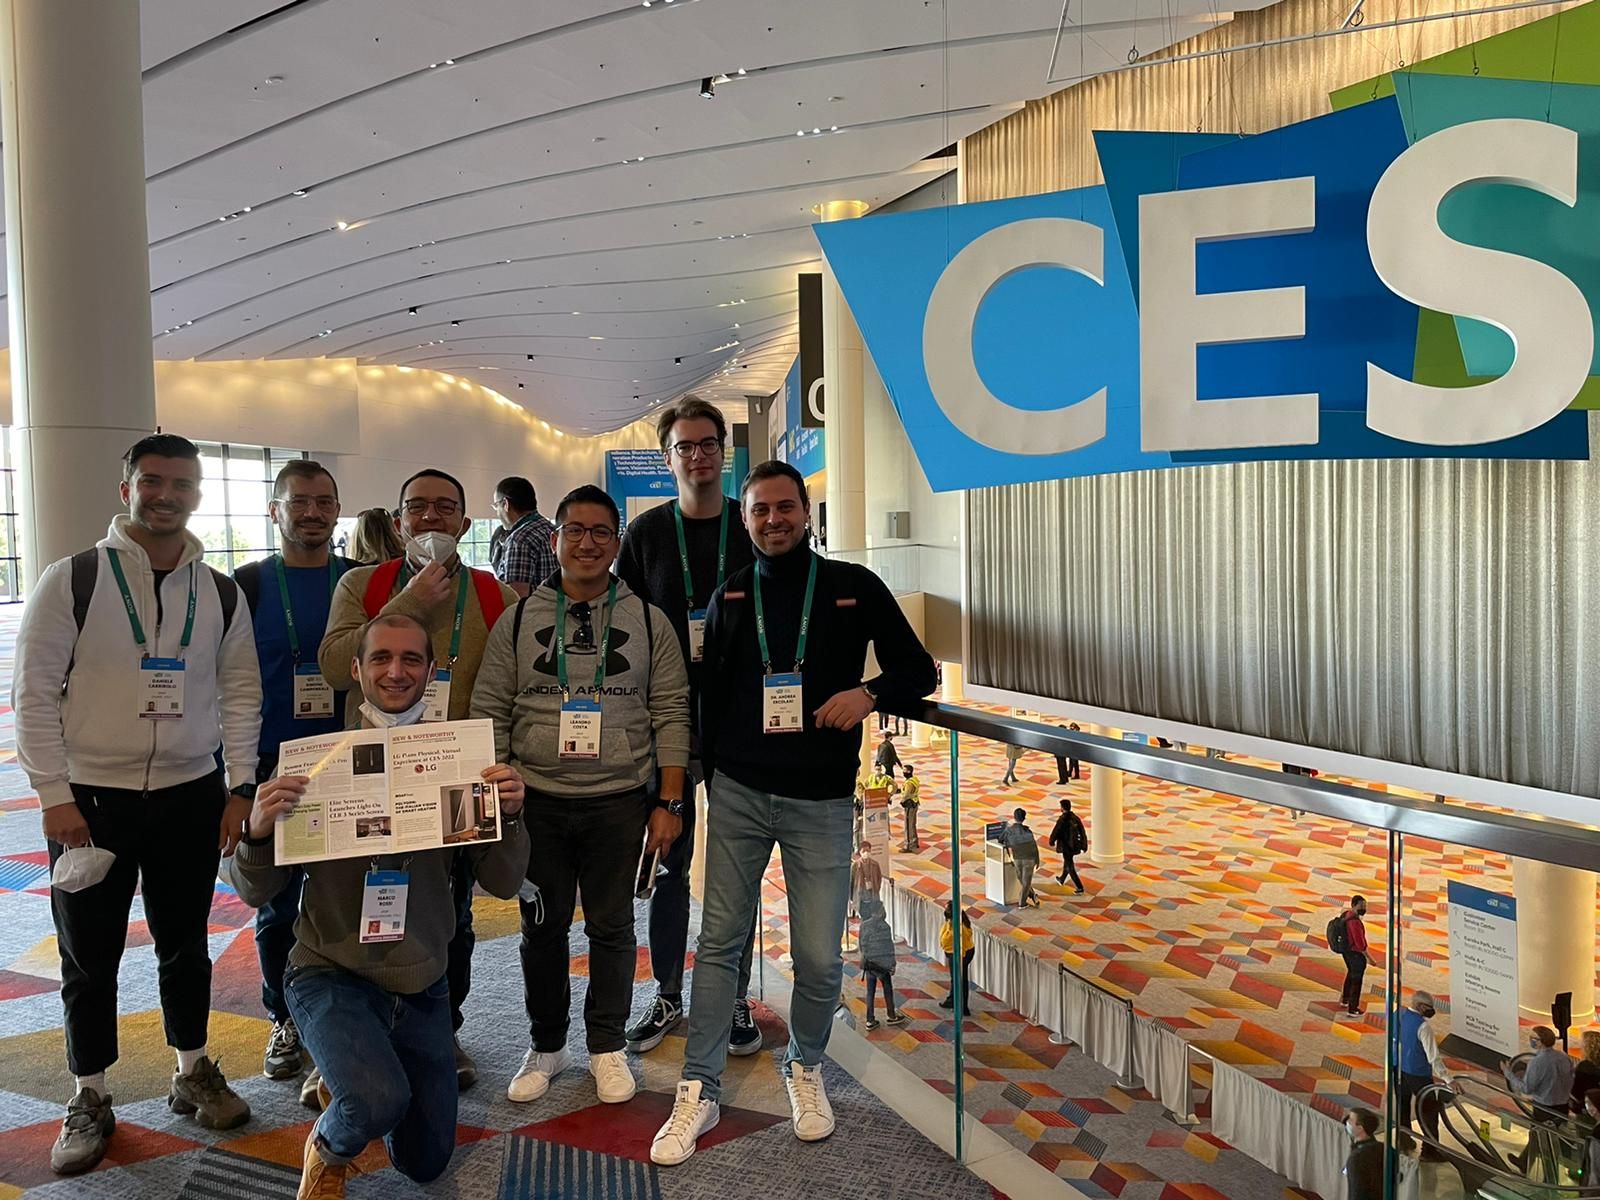
\includegraphics[width=12cm]{img/ces.jpeg}
    \caption{IRSAP ed IOTINGA al CES 2022}
    \label{fig:ces}
\end{figure}

\chapter{Definizione del problema}

Nessun utente installerebbe in casa propria un dispositivo che non è in grado di svolgere la funzione 
per la quale è stato acquistato, o che necessita di continue attenzioni.
A maggior ragione nessun venditore consiglierebbe ad un cliente un prodotto che funziona male, 
visto che poi è lui che ci mette la faccia e che deve fornire una garanzia al cliente riguardo 
al dispositivo che gli ha venduto. 

A maggior ragione il malfunzionamento di un impianto di riscaldamento può essere particolarmente 
fastidioso in quanto questo ricopre un ruolo fondamentale per il benessere domestico.

\section{Obblighi normativi}

Trattando prodotti destinati alla grande distribuzione e quindi all'acquisto da parte 
di privati si applica il \textit{codice del consumo}, che regolamenta i contratti di vendita
tra aziende e privati senza la necessità di negoziazioni in quanto diritti e doveri delle parti 
vengono stabiliti direttamente dalla legge italiana ed europea.

Esso stabilisce che le conseguenze legali legate alla sicurezza dei prodotti introdotti sul mercato 
sono a carico del \gls{produttore}, ovvero di colui che appone il proprio marchio sullo stesso. 
Invece la garanzia sui difetti di produzione, che in Italia ha durata minima di 2 anni, è a carico 
del venditore. Tuttavia il venditore, tramite accordi specifici, a sua volta si rivale solitamente 
sul produttore. 

In definitiva il principale responsabile della qualità e sicurezza dei prodotti è il produttore.

\section{Conseguenze economiche}

Per quanto concerne i danni accidentali, ad esempio un radiatore che perdendo acqua allaga la casa,
il produttore può tutelarsi avvalendosi di un'assicurazione, che, una volta appurato che il produttore
ha messo in atto tutte le misure preventive possibili, risarcisce il danno. 

Invece per quel che riguarda i difetti di fabbrica, che includono difetti del software, questi sono 
totalmente a carico del produttore, che è tenuto a correggerli o dove non sia possibile farlo a sostituire 
i prodotti difettosi con una campagna di richiamo. 

Dobbiamo tenere presente che il richiamo di un prodotto ha un costo molto elevato per il produttore, soprattutto 
nel nostro caso, in quanto trattando di prodotti di \textit{design} molto spesso nella loro spedizione per 
effettuare il reso questi vengono danneggiati in maniera irreparabili e devono quindi essere necessariamente 
sostituiti con un nuovo esemplare. 

Oltre ciò c'è il danno d'immagine, se l'utente è poco soddisfatto va a parlare male del prodotto, ed una 
recensione negativa è una macchia difficilissima da cancellare, una volta che il prodotto si è fatto la fama 
di essere poco affidabile non è semplice, se non è impossibile, rimediare. 

È quindi importantissimo per il produttore mettere in atto delle procedure tali da ridurre il più 
possibile la probabilità che questi difetti emergano.

\section{Prevenzione di danni fisici}

Per quanto concerne il prevenire danni fisici esistono leggi italiane e direttive europee che si applicano 
a determinate categorie di prodotti di elettronica di consumo. Nel nostro caso si applica, ad esempio, la
direttiva 2014/53/UE \acrshort{red}\footnote{\url{https://eur-lex.europa.eu/legal-content/IT/TXT/PDF/?uri=CELEX:32014L0053&from=lv}},
che ha campo di applicazione sui dispositivi elettronici in grado di 
effettuare comunicazioni radio (il che include l'uso del \Gls{wifi}). 

Lo scopo di leggi e direttive è fissare i principi generali che essenzialmente si riducono al dire che 
il prodotto deve essere progettato in una maniera tale che non possa, se usato nei modi e per gli scopi 
indicati dal produttore, arrecare danni a cose, persone, o animali domestici. 

Per poter commercializzare un prodotto all'interno dell'Unione Europea è necessario a rilasciare una 
\textit{dichiarazione di conformità} ed apporre sul prodotto il marchio \textbf{CE}. A differenza di 
quanto si creda comunemente, e di quanto avviene negli Stati Uniti, il marchio \textbf{CE} è 
un'autocertificazione del produttore, che dichiara assumendosene la responsabilità di aver realizzato 
il prodotto \textit{a regola d'arte}. 

Chiaramente il modo più semplice (ma non l'unico) che ha il produttore per dimostrare di aver seguito la
\textit{regola dell'arte} è il seguire durante la sua progettazione le \textit{norme di prodotto} che si 
applicano, dimostrandolo facendo eseguire dei test di laboratorio ad un ente terzo certificatore. 

Tuttavia non è sufficiente eseguire solamente dei test a campione: è anche necessario mettere 
in piedi una procedura per collaudare ogni esemplare che esce dalla fabbrica, proprio per evitare che vi siano 
difetti sistematici in un intero lotto di produzione. Questo si ottiene mediante procedure di \textit{quality testing}. 

Nel nostro caso questi test sono effettuati sia dal produttore della scheda elettronica, 
che collauda ogni scheda a livello elettrico e funzionale, sia da IRSAP stessa, che collauda ogni radiatore 
assemblato (elettronica più corpo scaldante) per verificare che funzioni correttamente e che non presenti 
pericoli (ad esempio dispersioni elettriche). 

\section{Prevenzione dei danni software}

E per quanto concerne il software? Purtroppo attualmente non esistono (ancora) obblighi normativi per 
i prodotti di \textit{elettronica di consumo} che impongano la realizzazione del software seguendo determinati 
standard. Essi esistono solo per settori specifici, come l'aereospaziale, il medicale, il militare, ecc. 

Il fatto che non esistano obblighi non significa che volontariamente un produttore non possa auto imporsi determinati 
standard internamente. Lo standard \acrfull{sil} è il più riconosciuto in ambito industriale per la valutazione 
della sicurezza del software ed è contenuto nella norma IEC 61508. 

Esso definisce 4 livelli, dal meno stringente (livello 1) al più restrittivo (4). Ogni 
livello presenta requisiti per quanto concerne la progettazione, lo sviluppo e la validazione 
del software realizzato, che sono riassunti nella seguente tabella:

\begin{center}
\begin{small}
\begin{longtable}{| p{0.18\textwidth} | p{0.18\textwidth} | p{0.18\textwidth} | p{0.18\textwidth} | p{0.18\textwidth} |}
    \hline
    \textbf{metrica} & \textbf{SIL 4} & \textbf{SIL 3} & \textbf{SIL 2} & \textbf{SIL 1} \\ \hline\hline
    Definizione delle specifiche e dei requisiti di progetto & Formale (descrizione strutturata e dettagliata dei comportamenti in linguaggio matematico) & Semi-Formale (descrizione strutturata e dettagliata dei comportamenti in linguaggio natural & Informale (descrizione in linguaggio naturale & Informale (descrizione in linguaggio naturale) \\ \hline
    Configuration-Management & Completa (automatica per sviluppo e produzione) & Completa (automatica per sviluppo e produzione) & Con l’ausilio di strumenti & Manuale \\ \hline
    Prototipazione & Si & Si & Opzionale & Opzionale \\ \hline
    Progettazione strutturata (uso di flow-chart, schemi relazionali o altro) & Si & Si & Preferenziale & Opzionale \\ \hline
    Verifica della progettazione & Si (da parte del team di progetto) & Si (da parte del team di progetto) & Si (da parte del team di progetto) & Si (esperti esterni) \\ \hline
    Project-Management & Si & Si & Si & Preferenziale \\ \hline
    Valutazione tecnica indipendente & Si & Preferenziale & Opzionale & Opzionale \\ \hline
    Analisi della gestione dei dati (necessaria per GDPR) & Si & Si & Si & Si \\ \hline
    Analisi Statistica (es. Unit Testing) & Si & Si & Opzionale & Opzionale \\ \hline
    Analisi Dinamica (es. Test automatici) & Si & Si & Si & Si \\ \hline
    Testing indipendente & Si (da org. esterna) & Si (da org. esterna) & Si (da Committente) & Opzionale \\ \hline
    Monitoraggio indipendente (test periodici) & Si (da org. esterna) & Si (da org. esterna) & Si (da Committente) & Opzionale \\ \hline
\end{longtable}
\end{small}
\end{center}

Nei progetti che sviluppiamo in IOTINGA utilizziamo solitamente il livello 2. 
Il limite principale dei livelli 3 e 4 è la definizione della specifica, che 
deve essere formale o semi-formale. I clienti solitamente ci forniscono le specifiche in linguaggio 
naturale, in quanto il fare diversamente sarebbe molto dispendioso in termini di tempo, 
e ciò poco si adatta con il modello di sviluppo \textit{agile} che seguiamo. 

Infatti i prodotti di elettronica di consumo devono rispondere velocemente alle esigenze del mercato, 
così da rimanere competitivi verso la concorrenza, e quindi devono essere sviluppati velocemente e poter 
evolvere durante la loro vita con l'aggiunta di nuove funzionalità per rimanere appetibili. 

I prodotti della precedente generazione utilizzavano il software per una sola gestione
delle periferiche fisiche del prodotto, senza la necessità di interfacciarsi con sistemi
terzi. Il software era quindi molto semplice, e una volta validato in laboratorio 
non c'erano grosse possibilità che smettesse di funzionare (salvo guasti hardware). 

Nella nuova generazione di prodotti invece l'hardware è più evoluto, passiamo ai \gls{micro} 
ad 8 bit quelli a 32-bit, con funzionalità sempre più assimilabili a quelle di un sistema
general purpose, quali ad esempio una gestione di programmazione concorrente tramite un \acrfull{rtos}, uno
stack di rete TCP/IP, ed una gestione della memoria virtual con MMU.

Un'altra differenza rispetto al passato è la possibilità di aggiornare il software dopo
che il prodotto lascia la fabbrica, mediante aggiornamenti di tipo \acrfull{ota}.
Questo si rende necessario non solo per l'introduzione di nuove funzionalità in
un prodotto esistente, ma anche per mantenere il software al passo con l'evoluzione degli
altri sistemi lato server a cui si collega, che nel tempo necessariamente evolvono a volte 
in maniera non retrocompatibili.

Bisogna infatti tener conto che un prodotto di questo tipo segue un ciclo di vita molto lungo
rispetto ad esempio a PC o smartphone, che può tranquillamente superare i 10 anni dalla data di
immissione nel mercato, e l'utente si aspetta che in tutti questi anni continui a funzionare. 
Sebbene la legge obblighi solo a garantire il funzionamento soltanto per il periodo di durata 
della garanzia, è chiaro che se il prodotto dopo 2 anni smette di funzionare come in origine 
il cliente sarebbe particolarmente arrabbiato e probabilmente per i prossimi acquisti si rivolgerebbe altrove. 

Non basta più quindi andare a validare il software una sola volta quando si fanno i test 
di laboratorio prima di immettere il prodotto sul mercato, ma la validazione deve essere continua, 
per tutta la vita del prodotto, per ogni singolo aggiornamento \acrfull{ota} che viene mandato 
ai dispositivi. 

\section{Prassi attuale di test}

Posto che il rischio zero è irraggiungibile è necessità del produttore mettere in campo 
tutte le procedure possibili per ridurre il più possibile la probabilità che i problemi 
sopracitati si verifichino.

Un ruolo fondamentale lo assumono quindi i test funzionali che si occupano di validare 
ogni rilascio firmware per il dispositivo. Questo è attualmente fatto in tre momenti:
\begin{enumerate}
    \item test durante lo sviluppo
    \item test di accettazione interna (effettuati da IOTINGA)
    \item test di accettazione del produttore (effettuati da IRSAP)
\end{enumerate}

\subsection{Test durante lo sviluppo}
\label{subsection:test_sviluppo}

Quando uno sviluppatore finisce di implementare una nuova funzionalità o risolve un
bug prima di poter considerare l'attività conclusa ed integrare il
proprio lavoro nel ramo di sviluppo principale è tenuto ad effettuare dei test.

Questi sono volti ad assicurare:
\begin{itemize}
    \item che le funzioni che prima c'erano continuino a funzionare come prima (test di regressione)
    \item che le eventuali nuove funzionalità aggiunte siano conformi alla specifica del cliente
    \item che gli eventuali i bug risolti non siano più presenti 
\end{itemize}

Questi test possono essere svolti sia in maniera automatizzata, ovvero tramite strumenti di 
\textit{unit testing}, che è il modo preferibile di procedere, sia manualmente, installando 
il software su un dispositivo. 

\subsection{Test di accettazione interna}
\label{subsection:test_accettazione_interna}

I test di accettazione interna si occupano di validare l'output finale del processo di sviluppo, 
il binario eseguibile, prima che arrivi nelle mani del cliente.  
Solo se una versione del software passa tutti questi test può essere consegnata al cliente.

Questi test si pongono dal punto di vista dell'utilizzatore finale e non entrano nel merito di come 
il codice è stato strutturato internamente, che viene trattato come una scatola chiusa. 

Attualmente vengono effettuati esclusivamente in maniera manuale, con il solo ausilio di un documento
di definizione contenente una serie di casi da testare. Per ognuno di essi è indicata una serie di 
passaggi, ognuno riportante:

\begin{itemize}
    \item azione da compiere: un'operazione da effettuare sul sistema mediante l'interazione fisica
        con il dispositivo (pressione di pulsanti) oppure mediante cloud (tramite un apposito
        strumento che consente di simulare i messaggi inviati dal cloud e dalla app)
    \item risultato atteso: postcondizioni da verificare dopo aver effettuato l'azione, espresso in
        linguaggio non formale, ad esempio ``i \acrshort{led} sono rossi'' oppure ``entro 5 secondi viene inviato al cloud un messaggio''.
        Nel caso la postcondizione sia verificata è possibile procedere al passo successivo, altrimenti
        il test viene interrotto con esito negativo, e deve essere segnalato ad uno sviluppatore il problema.
\end{itemize}

Per ogni passo chi esegue il test deve effettuare l'azione e verificare che il risultato atteso sia 
conforme a quanto indicato. Se così non è bisogna indicare a margine del documento cosa è andato 
storto, cercando di raccogliere quante più informazioni possibili per aiutare lo sviluppatore a replicare 
il problema per poi risolverlo. 

Una nota interessante è che questa procedura preferiamo farla eseguire a persone che non sono 
sviluppatori del progetto in questione. Questo per evitare che chi esegue la procedura, conoscendo
le logiche interne del software, possa essere portato a saltare o ignorare determinati
passaggi in quanto ``ovvi'', mentre chi non conosce il sistema è più propenso a seguire
i passaggi alla lettera e segnalare ogni singolo comportamento discordante con quanto
atteso.

\subsection{Test di accettazione del produttore}
\label{subsection:test_accettazione_produttore}

Sul \gls{produttore} ricade la responsabilità (legale) del prodotto
che viene immesso sul mercato con il proprio marchio sopra, e questo include anche
il software. Questo comporta il fatto che a sua volta deve svolgere dei test per
assicurarsi che il software sia conforme a quanto atteso, e nel caso segnalare i
problemi riscontrati in maniera tale che vengano corretti.

Questi test sono volti a testare tutte le funzionalità del prodotto in tutte le loro
possibili configurazioni, anche mediante l'ausilio di strumentazione altamente
specializzata quali camere climatiche per valutarne l'efficacia di termoregolazione.

Nel caso questi test abbiano successo l'artefatto testato passa da stato di candidato
al rilascio a produzione, e viene quindi installato in fabbrica su tutti i nuovi radiatori
prodotti, nonché viene lanciato un aggiornamento \acrshort{ota} su tutti i dispositivi già installati
presso i clienti finali.

\section{Problemi dell'approccio attuale}

Per la fase vista in \autoref{subsection:test_sviluppo} non ci sono particolari problemi,
come detto esistono una moltitudine di strumenti con i quali il lavoro può essere automatizzato. 

La fase in \autoref{subsection:test_accettazione_produttore} invece è piena responsabilità del 
\gls{produttore} che decide come meglio crede come svolgerla. 

La componente più critica ora è la fase in \autoref{subsection:test_accettazione_interna}. 
L'approccio attuale infatti presenta varie problematiche:
\begin{itemize}
    \item la procedura è ripetitiva, e questo può facilmente indurre
        l'operatore a commettere errori
    \item l'esecuzione della procedura richiede molto tempo, che potrebbe essere dedicato
        ad altre mansioni
    \item i test sono scritti in linguaggio naturale, non formale, e questo lascia un grado di 
        interpretazione all'operatore che svolge i test
    \item per quanto detto ai punti precedenti la procedura non può prendere in considerazione 
        tutti i possibili scenari, altrimenti sarebbe troppo lunga da eseguire, pertanto solo un 
        sottoinsieme di casi d'uso ``critici'' viene testata
    \item infine ancora per quanto sopra il numero di build effettivamente testate
        è un sottoinsieme di quelle prodotte, il che significa che
        i rilasci verso il cliente avvengono con meno frequenza, e si tende ad accorpare
        più funzionalità in maniera tale da effettuare un unico ciclo di test.
\end{itemize}

A questo si aggiunge il fatto che man mano che i prodotti arrivano nelle mani di sempre più consumatori 
il rischio per il produttore aumenta, e quindi viene richiesta sempre una maggiore qualità del software, 
che ci costringe ad effettuare sempre più test. 

La cosa positiva è che vista la definizione pressoché schematica e meccanica degli scenari da validare 
si potrebbe pensare di scrivere un software in grado di eseguirlo in maniera del tutto automatizzata, 
che possa richiedere un intervento umano nullo.

\section{Requisiti software per l'automazione}

Vediamo quindi i requisiti che questo sistema deve avere:

\begin{itemize}
    \item il sistema deve testare esattamente il binario che poi viene rilasciato agli utenti finali.
        Questo perché ogni alterazione, come potrebbe essere una ricompilazione del codice, può andare
        ad aggiungere errori e quindi invalidare i test effettuati
    \item l'ambiente di esecuzione (\textit{runtime environment}) sul quale il test viene eseguito deve essere quanto
        più vicino possibile all'ambiente reale. Idealmente il test viene effettuato sullo stesso hardware,
        di modo da dipanare ogni possibile dubbio che il \gls{firmware} una volta installato sull'hardware abbia
        comportamenti differenti
    \item l'ambiente deve poter eseguire il \gls{firmware} in differenti configurazioni di hardware che esso supporta
        (attualmente supporta due tipologie di hardware, e ne verranno aggiunte altrettante due a breve)
    \item il sistema deve avere abbastanza flessibilità per poter validare almeno le funzionalità che oggi
        sono teste manualmente
    \item deve essere sufficientemente semplice andare ad aggiungere nuovi scenari e configurazioni da provare al sistema
    \item deve essere possibile integrare lo strumento all'interno del flusso di CI attualmente in
        uso in azienda, di modo che ogni release del \gls{firmware} prodotta venga testata senza necessità di
        un intervento manuale
\end{itemize}

Osservato che sul mercato non esistono sistemi commerciali o open-source in grado di rispondere ai requisiti 
sopra elencati non ci rimane che svilupparne uno in casa. 

\chapter{Approccio}

Prima di descrivere l'implementazione è necessario fare un passo indietro ed andare
ad sviscerare il dispositivo \Gls{re} andando a vedere i dettagli più tecnici.

\section{Caratteristiche hardware}

Il corpo principale dei radiatori elettrici di IRSAP è del tutto identico al radiatore idraulico,
ed è realizzato mediante tubi d'acciaio saldati in un'unico corpo all'interno del quale circola 
il liquido termovettore, che tipicamente è l'acqua riscaldata da una caldaia o da una pompa di calore. 

Nel caso dell'elettrico viene inserita una resistenza elettrica, in gergo specifico \textit{cartuccia},
all'interno del radiatore, che viene riempito con del glicole, che a differenza della normale acqua 
ha un punto di congelamento più basso ed un punto di ebollizione più alto. Vengono infine sigillati 
tutti gli ingressi/uscite che normalmente consentirebbero il collegamento ad un impianto idraulico con dei tappi. 

Il cuore del sistema è poi la scheda elettronica di controllo che va ad alimentare la \textit{cartuccia},
e viene installata nella parte bassa del radiatore. 

\subsection{Scheda elettronica}

Attualmente la gamma di radiatori IRSAP elettrificati smart include 17 modelli distinti, 
ognuno dei quali disponibile in decine di colorazioni, ed ogni anno ne vengono aggiunti di nuovi. 

Per tutti questi dispositivi è quindi fondamentale, per ottimizzare i costi, avere un'elettronica 
unica. Attualmente vi è soltanto un'unica tipologia di scheda, che viene prodotta in due modelli 
leggermente diversi dal punto di vista fisico:

\begin{itemize}
    \item \textit{luxury}: è la versione più basilare, che viene utilizzata sulla linea di
        radiatori da bagno (chiamati anche ``scaldasalviette''). Essendo installata in ambiente 
        particolarmente umido e con il rischio di schizzi d'acqua deve sopportare un grado IP (
        misura standard del grado di protezione per componenti elettrici) superiore
    \item \textit{design} (\autoref{fig:schedadesign}): è la versione riservata ai prodotti design. È la più completa,
        che offre anche modularità essendo che tutte le periferiche (pulsantiera, sensore di temperatura,
        sensore VOC, \acrshort{led}) sono collegati alla stessa con dei cavi, il che consente di inglobarla
        all'interno della carcassa del \acrshort{re} in maniera da renderla invisibile, molto importante per non rovinare 
        il desing del prodotto. Offre inoltre funzionalità aggiuntive, quali un sensore di qualità
        dell'aria (in grado di rilevare i valori di VOC e CO\textsubscript{2}) e la possibilità di
        controllare una striscia \acrshort{led} \Gls{rgbw}, utilizzata su alcuni modelli per un'illuminazione ambientale.
\end{itemize}

Il modello \textit{luxury} è dal punto di vista delle caratteristiche hardware un sottoinsieme di quanto 
previsto dal modello superiore (\textit{design}). Entrambe montano:

\begin{itemize}
    \item un modulo \Gls{wifi} Telit GS2200M
    \item un circuito di alimentazione a tensione di rete (230V AC)
    \item un circuito composto da un relè combinato ad un triac dedicato al controllo di potenza, 
        ossia l'accensione e spegnimento della resistenza scaldante
    \item una sonda di temperatura \Gls{ntc} usata per misurare la temperatura ambiente
    \item una pulsantiera dotata di due pulsanti capacitivi e di \acrshort{led} RGB di illuminazione
        come feedback verso l'utente
    \item un buzzer utilizzato per un feedback uditivo della pressione dei pulsanti
    \item un circuito di lettura per il segnale \textit{\Gls{filpilote}} (il cavo nero collegato 
        in basso a destra nella scheda in \autoref{fig:schedadesign})
\end{itemize}

La versione \textit{design} include inoltre:
\begin{itemize}
    \item un sensore di qualità dell'aria in grado di misurare i livelli VOC e CO\textsubscript{2}
    \item la circuiteria di controllo per una striscia a \acrshort{led} \acrshort{rgbw} di illuminazione ambientale
        ed il relativo alimentatore da 230V AC a 24V DC
    \item la circuiteria di controllo per una seconda sonda di temperatura \acrshort{ntc} secondaria in grado di
        misurare la temperatura del corpo riscaldante, in maniera tale da migliorare
        l'accuratezza degli algoritmi di termoregolazione (solo per alcuni modelli)
\end{itemize}

\begin{figure}
    \centering
    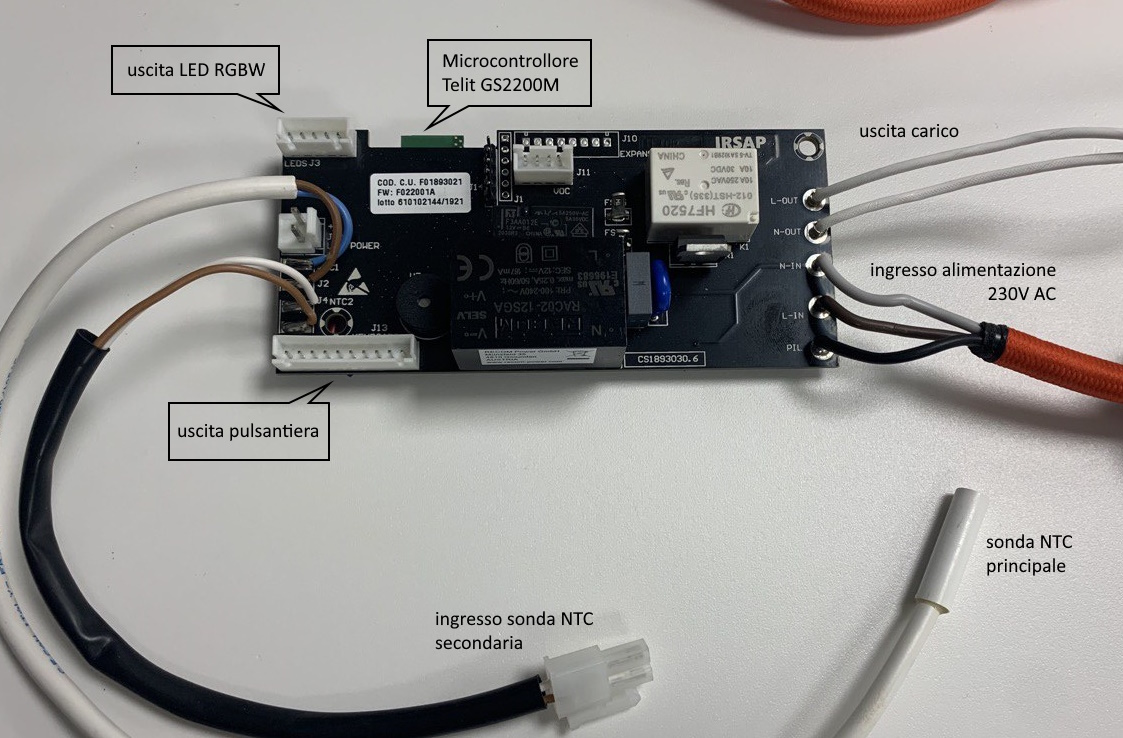
\includegraphics[width=\textwidth]{img/scheda-design.jpg}
    \caption{scheda elettronica modello \textit{design}}
    \label{fig:schedadesign}
\end{figure}
    
Vista la similarità entrambe le versioni di scheda elettronica eseguono la stessa versione del \gls{firmware},
che all'avvio identifica la tipologia di scheda tramite un file di configurazione caricato in fase di produzione
ed abilita/disabilita di conseguenza le periferiche opzionali. 

\subsection{Modulo Telit}

Il fulcro del sistema è il modulo \Gls{wifi} GS2200M. Questo \gls{micro}, inizialmente
prodotto da Gainspan e successivamente acquisita da Telit, presenta le seguenti
caratteristiche hardware:

\begin{itemize}
    \item processore dual core \Gls{arm} Cortex M3 fino a 120Mhz, di cui un core dedicato
        alla gestione del \Gls{wifi} ed uno all'esecuzione dell'applicativo
    \item 1Mb di RAM in totale, di cui all'incirca 500kB utilizzabile dall'applicazione,
        il resto dedicata all'uso della parte \Gls{wifi}
    \item 4Mb di memoria flash interna, in parte dedicata al codice del \gls{firmware} ed
        in parte come filesystem interno in cui memorizzare i dati dell'applicazione
    \item interfaccia \Gls{wifi} b/g/n a 2.4Ghz in grado di operare sia in modalità \Gls{sta} 
        sia che \Gls{ap} a cui connettersi direttamente
    \item 19 ingressi/uscite digitali \acrfull{gpio} 
    \item 3 output \acrfull{pwm}
    \item 2 ingressi analogici mediante \acrfull{adc}, uno a 10 ed uno a 12 bit
    \item un interfaccia \Gls{i2c} hardware
    \item un interfaccia \acrfull{spi} hardware
    \item due interfacce seriali \acrshort{uart}
    \item modulo \acrfull{rtc} interno
\end{itemize}

Il microcontrollore è dotato due due core \Gls{arm}, di cui uno è deputato alla gestione
della parte \Gls{wifi} ed esegue un \gls{firmware} scritto dal produttore stesso, l'altro 
invece è sotto il controllo dello sviluppatore. 

La toolchain fornita dal produttore si basa sull'ambiente di sviluppo proprietario IAR. Insieme 
a questa Telit fornisce un \acrfull{sdk} che offre:

\begin{itemize}
    \item un \Gls{rtos} basato su ThreadX
    \item uno stack di rete TCP/IP basato su NetX
    \item implementazione software \Gls{wifi} sia in modalità \acrfull{sta} che \acrfull{ap},
        con relativi protocolli WEP, WPA/WPA2 sia personal che enterprise
    \item un filesystem (simile a FAT32) per la gestione della memoria flash integrata
    \item implementazione \gls{tls}
    \item implementazione client e server del protocollo \acrshort{http} ed HTTPS
    \item implementazione client del protocollo \acrfull{sntp} 
    \item aggiornamento \acrshort{ota} con doppia partizione
    \item hardware abstraction layer (HAL) per la gestione di tutti i \Gls{gpio},
        lettura dei due \Gls{adc}, del modulo PWM, gestione del RTC, del bus i2c ed SPI
\end{itemize}

I moduli \Gls{wifi} di questo tipo generalmente possono essere utilizzati secondo due modalità:
\begin{itemize}
    \item \textit{hosted}: il modulo \Gls{wifi} viene interfacciato ad un microcontrollore
        principale che implementa le funzioni del dispositivo. Quest'ultimo si interfaccia
        con il Telit mediante interfaccia \acrshort{uart} e comunica con i comandi AT (standard
        per la gestione dei modem)
    \item \textit{hostless}: il modulo \Gls{wifi} esegue direttamente l'applicativo senza
        l'ausilio di un \gls{micro} principale. Tutte le funzionalità del dispositivo
        sono implementare sul modulo Telit
\end{itemize}

L'approccio più seguito è il primo approccio, tuttavia noi usiamo il secondo.
Questo offre svariate semplificazioni: non dobbiamo gestire la distribuzione
e l'aggiornamento \acrshort{ota} di due \gls{firmware} ed abbiamo più controllo sulla 
parte di \Gls{wifi}.

Un secondo microcontrollore comporta poi problemi di approvvigionamento, soprattutto di
questi tempi in cui il mercato dei componenti elettronici è impazzito è importante ridurre 
al minimo il numero di componenti critici utilizzati, quelli di difficile rimpiazzo, usati in un progetto.

La scelta di seguire l'approccio \textit{hostless} non è stata senza difficoltà, dovute
principalmente alla scarsa documentazione fornita dal produttore Telit. Infatti 
Telit ha deciso di seguire un approccio completamente closed-source, dove tutta
la documentazione ed il codice di esempio non è pubblico accessibile solo da area riservata.
Questo comporta che l'unico modo per risolvere i problemi sia quello di rivolgersi
al supporto ufficiale, non trovando nulla riguardo questa particolare piattaforma
hardware con una semplice ricerca su Google.

\section{Caratteristiche software}

Il \gls{firmware} sviluppato è suddiviso in moduli (ognuno dei quali gira in un \textit{thread} dedicato):

\begin{itemize}
    \item \textit{core}: implementa la macchina a stati che gestisce gli stati principali del dispositivo. 
        È il primo a partire e pertanto gestisce tutta la fase di inizializzazione del sistema, riceve e gestisce 
        gli eventi dagli altri moduli mediante una coda di messaggi.  
    \item \textit{termostato}: si occupa di tutto quel che concerne la regolazione della temperatura ambiente 
        secondo le modalità di funzionamento selezionata. Oltre a ciò effettua le letture delle sonde \acrshort{ntc}
        e VOC, e nei modelli che ne sono dotati gestisce anche i \acrshort{led} \acrshort{rgbw}, 
    \item \textit{\acrshort{aws}}: si occupa di mantenere attiva la connessione \Gls{mqtt} verso \Gls{iotcore},
        mantenendo sincronizzato lo stato interno del dispositivo con il server \Gls{now} attraverso il protocollo 
        \textit{stateless} che vedremo in seguito
    \item \textit{\acrshort{hmi}}, si occupa dell'interazione fisica con l'utente mediante l'input di due pulsanti \textit{+} e 
        \textit{-}, e l'output dei \acrshort{led} di stato e del buzzer. In base agli input dell'utente invia i relativi 
        messaggi agli altri moduli
    \item \textit{\acrshort{http}}, si occupa di fornire mediante webserver \acrshort{http} un'API REST con
        la quale è possibile interagire direttamente con il dispositivo. È utilizzata principalmente durante per 
        la fase di abbinamento del dispositivo con la app, ma ha anche funzioni di diagnostica.
    \item \textit{\acrfull{ncm}}, si occupa di gestire la connessione di rete \Gls{wifi}. 
\end{itemize}

\subsection{Stati interni del dispositivo}

Il dispositivo ad alto livello (\textit{core}) può trovarsi in 3 stati:

\begin{itemize}
    \item \textit{non abbinato}: in attesa di un primo abbinamento da app. Ogni funzione del
        dispositivo è disabilitata finché l'utente non lo collega mediante l'applicazione
    \item \textit{disconnesso}: il dispositivo è stato in passato abbinato ma al momento non è
        connesso al cloud, perché ad esempio la connessione \Gls{wifi} non è momentaneamente disponibile
    \item \textit{connesso}: il dispositivo è connesso e sincronizzato con il cloud, è la modalità di funzionamento usuale
\end{itemize}

\begin{figure}[ht]
    \centering
    \begin{tikzpicture}
        \node[state] (unbounded) {Non abbinato};
        \node[state, below left of=unbounded, below=1cm] (offline) {Disconnesso};
        \node[state, right of=offline] (online) {Connesso};
        \draw (unbounded) edge[bend left, align=left, right] node{abbinato\\con successo} (online)
        (offline) edge[bend left, above] node{connessione} (online)
        (offline) edge[bend left, left, align=right] node{ripristino\\di fabbrica} (unbounded)
        (online) edge[bend left, below] node{disconnessione} (offline)
        (online) edge[bend left, align=right, right] node{ripristino\\di fabbrica} (unbounded);
    \end{tikzpicture}
    \caption{Stati del radiatore}
    \label{fig:stati}
\end{figure}

Ad ogni stato del dispositivo corrisponde l'attivazione/disattivazione di uno o più
moduli:

\begin{center}
\begin{tabular}{| c | c | l |}
    \hline
    stato & modo \Gls{wifi} & moduli attivi \\ \hline
    \textit{non abbinato} & \acrshort{ap} & core, \acrshort{ncm}, \acrshort{hmi}, \acrshort{http} \\ \hline
    \textit{disconnesso} & \acrshort{sta} & core, \acrshort{ncm}, \acrshort{hmi}, termostato \\ \hline
    \textit{connesso} & \acrshort{sta} & core, \acrshort{ncm}, \acrshort{hmi}, termostato, \acrshort{aws} \\ \hline
\end{tabular}
\end{center}

\subsection{Termoregolazione}

Il modulo di termoregolazione si occupa di regolare la temperatura ambiente cercando di mantenerla
uguale a quanto desiderato dal consumatore (set-point). Questo avviane comandando l'accensione della 
resistenza in modo on/off. Il feedback sulla temperatura ambiente è ottenuto grazie alla sonda \acrshort{ntc} principale.

Il dispositivo ha diversi modi di funzionamento, in ordine di priorità:
\begin{itemize}
    \item \textit{standby}: dispositivo completamente spento, sia per quanto riguarda il riscaldamento
    che per l'illuminazione \acrshort{led}
    \item \textit{\gls{filpilote}}: il dispositivo è controllato da un segnale
        esterno in ingresso sul cavo \Gls{filpilote}
    \item \textit{antigelo}: il dispositivo mantiene una temperatura di sicurezza (impostata dall'utente)
        per prevenire danni alla casa ed al dispositivo causati da una temperatura ambiente troppo bassa
    \item \textit{vacanza}: funziona all'interno di un intervallo impostato fra due timestamp di inizio e di 
        fine come in modalità \textit{antigelo}
    \item \textit{away}: imposta un set-point ridotto (ECO) in quanto l'utente non è in casa
    \item \textit{manuale temporaneo}: segue un set-point manuale impostato dall'utente fino al raggiungere 
        un timestamp di fine
    \item \textit{programmato}: segue una programmazione settimanale che consente per ogni
        giorno della settimana di creare fino ad 8 fasce orarie
    \item \textit{manuale}: segue il set-point utente che è fisso e non varia mai
        configurato dall'utente, quindi torna a funzionare nella modalità precedente
\end{itemize}

Tutti i modi sopraelencati sono attivabili tramite app. Invece tramite pulsantiera del dispositivo è possibile 
muoversi nelle modalità \textit{manuale a tempo} oppure \textit{manuale} secondo lo schema in \autoref{fig:modi}.

\begin{figure}[ht]
    \centering
    \begin{tikzpicture}
        \node[state, minimum size=3cm] (programmato) {Programmato};
        \node[state, minimum size=3cm, right of=programmato, align=center] (manuale-tempo) {Manuale\\temporaneo};
        \node[state, minimum size=3cm, right of=manuale-tempo] (manuale) {Manuale};
        \draw (manuale) edge[loop above] node{interazione} (manuale)
            (programmato) edge[bend left, above] node{interazione} (manuale-tempo)
            (manuale-tempo) edge[bend left, above] node{interazione} (manuale);
    \end{tikzpicture}
    \caption{cambiamento di modi tramite tastiera}
    \label{fig:modi}
\end{figure}

\subsection{Comunicazione cloud}

Il dispositivo come anticipato si collega al \gls{cloud} \Gls{now}. La componente server è 
realizzata su piattaforma \Gls{aws} attraverso l'uso di tecnologie \gls{serverless}, che consentono 
al sistema di poter scalare in base al carico effettivo dinamicamente. 

Il protocollo di comunicazione usato dal dispositivo è \Gls{mqtt}, ed il \gls{broker} al quale 
viene collegato è \Gls{iotcore}. 

\subsubsection{Autenticazione}

La connessione è protetta mediante \acrshort{tls} 1.2 ed autenticata tramite l'utilizzo di un certificato \acrshort{tls} client.

Questo certificato è univoco per ogni singolo dispositivo ed è salvato all'interno del suo filesystem
durante la produzione dell'elettronica. Il certificato non è emesso direttamente da \acrshort{aws} ma 
è generato attraverso una \acrfull{ca} intermedia del produttore delle elettroniche come in \autoref{fig:tls-chain}. 
Questo consente di poter generare dei certificati ``offline'' durante le fasi di produzione, in cui non 
è sempre garantita una connessione ad internet, sia consentirebbe di generare il certificato direttamente 
sul dispositivo andando a far sì che la chiave \textit{privata} non sia mai nota al produttore. 

\begin{figure}[ht]
    \centering
    \begin{tikzpicture}
        \node[rectangle, draw, align=center, inner sep=8pt] (root) {root \acrshort{ca} \\ \Gls{mqtt}};
        \node[rectangle, draw, right of=root, align=center, inner sep=8pt] (intermedia) { \acrshort{ca} intermedia\\ produttore};
        \node[rectangle, draw, right of=intermedia, align=center, inner sep=8pt] (dispositivo) {certificato \gls{tls}\\ dispositivo};
        \draw (root) edge[above] node{firma} (intermedia)
            (intermedia) edge[above] node{firma} (dispositivo);
    \end{tikzpicture}
    \caption{Catena \gls{tls}}
    \label{fig:tls-chain}
\end{figure}

La registrazione presso \Gls{iotcore} del dispositivo avviene quando questo si collega per la prima 
volta, che nel nostro caso corrisponde alla prima accensione della scheda elettronica durante il collaudo 
presso il produttore elettronico. A questo punto tramite delle regole viene automaticamente collegata 
una o più \textit{policy} al dispositivo, che gli danno i permessi per effettuare le operazioni fondamentali 
necessarie per la comunicazione su \gls{cloud}:

\begin{itemize}
    \item \textit{connect}: autorizza il client a connettersi ad \Gls{iotcore} utilizzando il \textit{clientId}
        corrispondente al proprio indirizzo MAC
    \item \textit{publish}: consente al client precedentemente autenticato di pubblicare i messaggi sui topic ad 
        esso riservati, ovvero i \gls{topic} con prefisso \textrm{re/things/\{MAC\}}
    \item \textit{subscribe}: consente al dispositivo di sottoscriversi per gli aggiornamenti ai topic a lui dedicati, 
        ovvero i \gls{topic} con prefisso \textrm{re/things/\{MAC\}}
\end{itemize}

\subsubsection{Protocollo stateless di comunicazione}

Per quanto concerne il protocollo di comunicazione abbiamo valutato inizialmente
l'uso del protocollo Device Shadowing\footnote{\url{https://docs.aws.amazon.com/it\_it/iot/latest/developerguide/iot-device-shadows.html}}
nativamente supportato da \Gls{aws} \Gls{iotcore}.

Tale protocollo aveva delle limitazioni che non ne consentivano l'utilizzo nella nostra
applicazione, in particolare:

\begin{itemize}
    \item il pacchetto viene codificato in \acrshort{json}, la cui gestione richiede memoria
        e tempo CPU non trascurabile per un dispositivo embedded
    \item \Gls{iotcore} ha un hard-limit di 8Kb di dimensione massima di un documento di stato (shadow).
        Questo, seppur poteva essere sufficiente nelle prime versioni del prodotto, andava
        a limitare le possibilità di futura espansione futura
    \item il protocollo di comunicazione trasferisce dei delta, che sebbene riducano la
        dimensione di un pacchetto di dati rendono più complessa la gestione sia lato dispositivo 
        sia lato server
\end{itemize}

Per questo abbiamo scelto di definire un nostro protocollo binario \textit{stateless},
tramite il quale andiamo a trasferire stati completi del dispositivo.

Abbiamo deciso di mantenere per convenzione i concetti di alto livello del protocollo \Gls{aws}
Device Shadowing, in particolare la nomenclatura \textit{shadow} per indicare uno stato \textit{completo} del
dispositivo, che si divide in:
\begin{itemize}
    \item \textit{state desired}: lo stato voluto del dispositivo. Include tutte quelle variabili di stato 
        che definiscono una configurazione del dispositivo, quali i parametri per la termoregolazione.
    \item \textit{state reported}: lo stato rilevato dal dispositivo. Include, oltre a tutte le variabili 
        di stato dello \textit{state desired} anche tutte le variabili contenenti dati statistici e di monitoraggio,
        quali temperatura ambiente, valori VOC e CO\textsubscript{2}, qualità della connessione \Gls{wifi}, allarmi, ecc. 
\end{itemize}

Attualmente sono previste dal protocollo 4 tipi di richieste, ognuna delle quali consente di eseguire un'azione verso 
il dispositivo o verso il \gls{cloud} (come visibile in \autoref{fig:comunicazione_cloud}):

\begin{itemize}
    \item \textit{get}: il dispositivo richiede al \gls{cloud} l'ultimo stato \textit{desired}
    \item \textit{delete}: il dispositivo richiede al \gls{cloud} di eliminare lo stato corrente
    \item \textit{reported-update}: il dispositivo invia al \gls{cloud} lo stato \textit{reported} corrente
    \item \textit{desired-update}: il \gls{cloud} notifica al dispositivo che vi è un nuovo stato \textit{desired}
\end{itemize}

Il tipo di messaggio dipende dal \gls{topic} sul quale i pacchetti sono pubblicati. Ad
un messaggio pubblicato dal dispositivo verso il \gls{cloud} segue una risposta sullo stesso \gls{topic}
con aggiunto un suffisso che indica l'esito dell'operazione:
\begin{itemize}
    \item \texttt{/accepted}: la richiesta ha avuto successo
    \item \texttt{/rejected}: la richiesta ha generato un errore, che è indicato nel payload della risposta
\end{itemize}

\begin{figure}[ht]
    \centering
    \begin{tikzpicture}
        \node[rectangle, minimum height=1cm, draw] (dispositivo) {\Gls{re}};
        \node[rectangle, minimum height=1cm, draw, right of=dispositivo] (cloud) {\Gls{iotcore}};
        \draw (dispositivo) edge[bend left=60, above] node{\textit{reported-update}} (cloud)
            (dispositivo) edge[bend left=20, above] node{\textit{get}} (cloud)
            (dispositivo) edge[bend right=20, below] node{\textit{delete}} (cloud)
            (cloud) edge[bend left=60, below] node{\textit{desired-update}} (dispositivo);
    \end{tikzpicture}
    \caption{Schema di comunicazione dispositivo/cloud}
    \label{fig:comunicazione_cloud}
\end{figure}

\subsubsection{Formato messaggi cloud}

Ogni messaggio su cloud include un header sempre uguale, che include i seguenti campi

\begin{center}
\begin{longtable}{| p{5cm} | c | p{8cm} |}
    \hline
    \textbf{chiave} & \textbf{tipo} & \textbf{descrizione} \\ \hline
    timestamp & u32 & timestamp di generazione del messaggio \\ \hline
    clientToken & u32 & identificativo della richiesta aggiunto dal richiedente. Nelle risposte 
        viene riportato questo valore senza variarlo, in maniera tale che il richiedente possa 
        capire a quale richiesta una risposta di riferisce \\ \hline
    version & u32 & versione dello stato. Viene incrementata ad ogni modifica dello stato \textit{desired} 
        da parte della app \\\hline
    length & u16 & lunghezza totale del messaggio in byte (header incluso) \\ \hline
    type & u8 & tipologia di messaggio inviata \\ \hline
\end{longtable}
\end{center}

Per i messaggi che prevedono dei dati sono aggiunti questi parametri (alcuni di questi 
parametri sono presenti solo nello stato \textit{reported}, altri sia nel \textit{desired} che nel \textit{reported}):

\begin{center}
\begin{longtable}{| p{5cm} | c | p{8cm} |}
    \hline
    \textbf{chiave} & \textbf{tipo} & \textbf{descrizione} \\ \hline
    connected & u8 & 1 se il dispositivo è online, altrimenti 0 \\ \hline
    firmwareVersion & u8[2] & versione \gls{firmware} (major, minor) \\ \hline
    hardwareVersion & u8 & versione hardware \\ \hline
    macAddress & u8[6] & MAC address (seriale del dispositivo) \\ \hline
    systemStatus & u8 & stato del Sistema (bitmask) \\ \hline
    filPiloteStatus & u8 & stato ingress Fil Pilote \\ \hline
    alarm & u8 & allarmi (bitmask)\\ \hline
    heatingStatus & u8 & stato riscaldamento (bitmask)\\ \hline
    RSSI & u8 & Potenza \Gls{wifi}\\ \hline
    noise & u8 & Rumore \Gls{wifi}\\ \hline
    currentSetPoint & i16 & set point corrente (in decimi di grado)\\ \hline
    currentSetPointEnd & u32 & scadenza set-point corrente\\ \hline
    vocValue & u16 & valore VOC (qualità dell’aria)\\ \hline
    co2Value & u16 & valore CO2 (qualità dell’aria)\\ \hline
    temperature & i16 & temperature ambiente (in decimi di grado)\\ \hline
    setPointOff & u16 & set point di OFF (espresso in decimi di grado)\\ \hline
    setPointEco & u8 & set point di ECO (espresso in decimi di grado - 10C)\\ \hline
    manualSetPoint & u8 & set point manual (espresso in decimi di grado -10C)\\ \hline
    temporaryManualSetPoint & u8 & set point manual temporaneo (in decimi di grado)\\ \hline
    temporaryManualEnd & u32 & fine manuale temporaneo (timestamp)\\ \hline
    hysteresis & u8 & isteresi (espressa in decimi di grado)\\ \hline
    temperatureSensorOffset & i8 & correzione sensore di temperature (espresso in decimi di grado)\\ \hline
    loadTemperature & i16 & temperature carico (in decimi di grado)\\ \hline
    loadOnSeconds & u32 & cumulativo in secondi di accensione del carico\\ \hline
    holidayStart & u32 & timestamp inizio vacanza\\ \hline
    holidayEnd & u32 & timestamp fine vacanza\\ \hline
    metricInterval & u8 & intervallo invio metriche periodiche (minuti)\\ \hline
    systemId & u8[16] & ID impianto (UUID)\\ \hline
    timezone & i16 & offset timezone rispetto ad orario UTC\\ \hline
    systemConfiguration & u8 & configurazione di sistema (bitmask)\\ \hline
    ipAddress & u8[4] & indirizzo IP \Gls{wifi}\\ \hline
    openWindowOffTime & u8 & tempo di spegnimento in caso rilevamento finestra aperta\\ \hline
    ledManualSetPoint & u32 & colore \acrshort{led} ambiente (HSV)\\ \hline
    schedule & u8[196] & programmazione riscaldamento\\ \hline
    ledSchedule & u8[196] & programmazione \acrshort{led} (stesso formato di prima)\\ \hline
    ledEnabled & u8 & \acrshort{led} ambiente on/off\\ \hline
    ledMode & u8 & modalità led ambiente (manuale/programmato)\\ \hline
    ledColor & u32[10] & preset colori \acrshort{led} ambiente per uso in fasce orarie\\ \hline
    temporaryManLedSP & u32 & set point \acrshort{led} manuale a tempo\\ \hline
    temporaryManLedSPEnd & u32 & fine manuale a tempo \acrshort{led}\\ \hline
    estimatedTemperature & i16 &temperatura ambiente (scritta da cloud per uso con altri sensori)\\ \hline
    externalTemperature & i16 & umidità esterna (scritta da cloud)\\ \hline
    estimatedHumidity & u8 & umidità ambiente (scritta da cloud)\\ \hline
    externalHumidity & u8 & umidità esterna (scritta da cloud)\\ \hline
    currentLedSetPoint & u32 & set point \acrshort{led} corrente\\ \hline
    currentLedSetPointEnd & u32 & fine fascia oraria \acrshort{led} corrente\\ \hline
    cartridgePowerWatts & u16 & potenza della cartuccia\\ \hline
    totConsumption & u32 & consumo cumulato in tutta la vita del radiatore\\ \hline
    totConsumptionValue & u32 & valore all’ultimo snapshot di consumo\\ \hline
    totConsumptionTime & u32 & consumo all’ultimo snapshot\\ \hline
    modelName & char[32] & nome modello del radiatore\\ \hline
\end{longtable}
\end{center}

\subsection{API di configurazione locale}

Quando il dispositivo viene acceso per la prima volta è necessario fornirgli la
configurazione della rete \Gls{wifi} e l'identificativo (UUID) dell'impianto al quale
collegarsi prima che esso possa iniziare a funzionare tramite la app \Gls{now}.

Questo avviene tramite \Gls{wifi} in quanto il modulo GS2200M non dispone di interfaccia 
\acrshort{ble}. Il cellulare effettua una connessione ad una rete \Gls{wifi} il cui 
SSID inizia con il prefisso di IRSAP (\texttt{IRSAP\_}). Dopo di che può chiamare 
le seguenti API REST implementate dal dispositivo:

\begin{center}
\begin{tabular}{| l | c | p{6cm} |}
    \hline 
    \textbf{endpoint} & \textbf{metodo} & \textbf{descrizione} \\ \hline 
    \texttt{/irsap/state} & GET & ottiene informazioni sul dispositivo \\ \hline 
    \texttt{/irsap/wifi/scan} & GET & ottiene l'elenco di reti \Gls{wifi} visibili dal dispositivo \\ \hline 
    \texttt{/irsap/provision} & POST & invia al dispositivo la configurazione \\ \hline 
    \texttt{/irsap/test} & POST & attiva la modalità collaudo del dispositivo \\ \hline 
    \texttt{/gainspan/system/fwup} & POST & invia un aggiornamento \gls{firmware} al dispositivo \\ \hline
\end{tabular}
\end{center}

Il flusso di abbinamento funziona pertanto nel seguente modo:
\begin{itemize}
    \item il cellulare si collega all'\acrshort{ap} messo a disposizione dal \acrshort{re}
    \item si chiama prima l'API \texttt{/irsap/state} per identificare la tipologia di dispositivo
    \item se dovesse essercene l'esigenza la app invia al dispositivo un aggiornamento \acrshort{ota} locale, 
        quindi attende che il dispositivo si aggiorni e si riconnette, ricominciando questa procedura da capo.
    \item nel caso si sia identificato un dispositivo \acrshort{re} (la stessa API sarà in futuro 
        usata da più dispositivi della famiglia \Gls{now} come gli impianti \acrshort{vmc}) chiama 
        l'API \texttt{/irsap/wifi/scan} per effettuare una scansione delle reti\footnote{questo si rende
        necessario poiché per questioni di privacy i cellulari con sistema operativo iOS non hanno accesso all'elenco 
        delle reti visibili dal dispositivo}
    \item dopo aver chiesto all'utente di scegliere una delle reti restituite dalla scansione e di 
        averne chiesto la passphrase, qualora fosse richiesta, invia una richiesta \texttt{/irsap/provision}
        al \acrshort{re} per completare l'abbinamento 
    \item a questo punto il \acrshort{re} si riavvia e prova a connettersi alla rete, mentre la app resta 
        in attesa di ricevere tramite \gls{cloud} una prima comunicazione dal \acrshort{re}
\end{itemize}

\subsection{Interfaccia utente}

La \acrfull{hmi} del dispositivo permette di interagire con l'utilizzatore mediante:
\begin{itemize}
    \item due pulsanti capacitivi, \textbf{+} e \textbf{-}
    \item dei led \acrshort{led} RGB di illuminazione dei pulsanti 
    \item un buzzer in grado di dare un feedback acustico ad ogni tocco della pulsantiera
\end{itemize}

Attraverso i due pulsanti è possibile comandare diverse operazioni:

\begin{itemize}
    \item pressione breve \textbf{+}: incrementa il set-point corrente (se \acrshort{re} in modo \textit{manuale} o \textit{manuale a tempo})
    \item pressione breve \textbf{-}: decrementa set-point corrente (se \acrshort{re} in modo \textit{manuale} o \textit{manuale a tempo})
    \item pressione per un tempo compreso fra 3 e 5 secondi del tasto \textbf{-}: attiva modalità \textit{antigelo}
    \item pressione per più di 5 secondi del tasto \textbf{-}: attivazione modalità \textit{stand-by}
    \item pressione prolungata dei tasti \textbf{+} e \textbf{-} per più di 5 secondi: avvia la procedura di ripristino impostazioni 
        di fabbrica (\textit{factory reset})
\end{itemize}

I \acrshort{led} invece sono utilizzati sia per segnalare la temperatura impostata dall'utente
(in base al set-point passano da un colore più freddo ad uno più caldo) mentre viene modificata la 
temperatura impostata, sia per indicare condizioni particolari quali radiatore non abbinato (\acrshort{led} rossi), connessione
in corso (viola lampeggiante), modo \textit{stand-by} (viola fisso) o \textit{antigelo} (bianco).

\section{Interfacciamento con il sistema di test}

Dalle sezioni precedenti possiamo riassumere che ad alto livello il \acrshort{re} interagisce con 
l'ambiente esterno attraverso 3 interfacce:

\begin{enumerate}
    \item \gls{cloud}: invio e ricezione di stati completi (\textit{shadow}) tramite \Gls{mqtt} ad \acrshort{aws} \Gls{iotcore}
    \item API locale: metodi messi a disposizione mediante il server HTTP REST del \acrshort{re}
    \item fenomeni fisici: calore emesso, pulsanti che vengono premuti, luce e suoni emessi, temperatura che cambia, ecc
\end{enumerate}

Riguardo ai primi due punti si possono usare strumenti ``convenzionali'' per automatizzare programmaticamente
le interazioni. Esistono diversi strumenti per farlo che sono comunemente utilizzati. 
La complessità quindi sta nelle interazioni fisiche con il dispositivo. Possiamo pensare di affrontare il problema in 3 modi:

\begin{itemize}
    \item interazione hardware con il prodotto finito
    \item interazione hardware con la scheda elettronica
    \item esecuzione del \gls{firmware} in un emulatore
\end{itemize}

\subsection{Interazione con il dispositivo fisico}

Possiamo immaginare di prendere un radiatore, sistemarlo in un ambiente attrezzato per 
modificarne le condizioni (come una camera climatica a temperatura controllabile) e dotato 
di sensori per misurare il comportamento del dispositivo. A questo punto possiamo collegare degli 
attuatori per eseguire automaticamente le operazioni che l'utilizzatore può fare sul \acrshort{re}. 

Questo ci garantisce di testare uno scenario del tutto identico, o comunque quasi identico, a quello  
che si trova nelle case dei consumatori finali. Tuttavia l'approccio presenta una serie di problematiche 
che lo rendono impraticabile:
\begin{itemize}
    \item è necessaria strumentazione molto specifica e costosa (le camere climatiche),
        che sebbene a disposizione di IRSAP sono occupate per altri scopi. Inoltre le misurazioni che si 
        possono effettuare hanno i limiti dati dall'osservabilità dei fenomeni fisici, che comporta un 
        inevitabile errore di misura che limita la precisione del test

    \item i test dovrebbero seguire le tempistiche dettate dai fenomeni fisici che si vanno a stimolare, 
        come il riscaldamento di un ambiente. Questo rende il test molto lungo in termini temporali, 
        rendendo necessari giorni per poter validare una versione firmware. Questo limita il numero di 
        versioni che si possono realisticamente testare e rallenta l'intero flusso di rilasci. 
\end{itemize}

\subsection{Interazione con la sola elettronica}

Viene da pensare che si possa quindi ridurre all'osso il \acrshort{re} andando ad eliminare tutte 
quelle componenti che hanno un impatto marginale o nullo sul software, che è l'oggetto dei nostri test. 

Ci rendiamo conto che non è necessario prendere in esame l'intero radiatore, che è un corpo meccanico, 
ma si può concentrarsi sulla sola scheda elettronica, andando a simulare gli ingressi/uscite digitali/analogici
con la quale interagisce con l'esterno. 

Notato questo, possiamo anche fare un passo ulteriore, e rimuovere completamente anche l'elettronica, 
andando a testare solo il microcontrollore, che è l'unica componente del sistema sulla quale vi è un software 
in esecuzione. Questo semplifica ulteriormente le cose, dato che le schede elettroniche sono alimentate 
con tensione di rete (230V AC nominale) che renderebbe quindi necessario isolare le schede sia per questioni 
di sicurezza che per evitare danni alle apparecchiature collegate. 

L'eliminare il fattore scheda elettronica non causa alcun problema, essendo che l'hardware viene già 
collaudato, come detto all'inizio del capitolo 2, durante la produzione in fabbrica. Gli scopi infatti 
di questa fase di test è la validazione di un software assumendo che l'ambiente di esecuzione funzioni 
come da specifica hardware. 

Possiamo quindi isolare solo la parte che ci interessa, ovvero il chip Telit, utilizzando
un kit di sviluppo fornito direttamente dal produttore. Questo permette di connettere
la nostra interfaccia di test con tutti gli input/output digitali (\Gls{gpio}) ed analogici della scheda,
così che potremo andare a simulare tutte le periferiche hardware più agevolmente via software.

Questa è la soluzione che alla fine ho scelto.

\subsection{Esecuzione del firmware in un emulatore}

Vediamo infine un'ultima possibilità, quella di eseguire il \gls{firmware} non sull'hardware
reale ma su un sistema emulato.

Questo presenta alcune problematiche nel nostro caso. In primis è difficile realizzarlo sulla piattaforma 
hardware Telit, essendo proprietaria è difficile ottenere tutte le specifiche di funzionamento per andare
ad emularne in maniera quanto più simile possibile il funzionamento. Su altri microcontrollori (ad esempio 
il popolare Espressif ESP-32) è possibile con il software di emulazione QEMU andare a simulare il microcontrollore 
in maniera molto fedele all'originale. 

Si potrebbe quindi decidere di compilare un binario x86, andando a sostituire tutte
le funzioni utilizzate del framework Telit con stub implementati ex-novo. Questo
sebbene potrebbe funzionare (anche se il suo sviluppo sarebbe molto lungo e dispendioso)
avrebbe come effetto che non si sta effettivamente testando il binario che poi andrà
in produzione, che era uno dei requisiti che avevamo stabilito all'inizio.

In secondo luogo l'emulazione comunque non è del tutto adatta a test di accettazione, in quanto non va veramente 
a validare l'interazione del software con l'hardware reale, e soprattutto quando si parla di interfacce radio 
come il \Gls{wifi} il comportamento potrebbe essere particolarmente diverso. A titolo di esempio infatti 
uno dei bug principali che abbiamo avuto sul \acrshort{re} era proprio l'incompatibilità con alcuni tipi di \acrlong{ap}
\Gls{wifi}, una condizione che sarebbe stata impossibile da diagnosticare senza far girare il software su hardware fisico.

\section{Conclusioni}

Concludiamo quindi stabilendo che il modo migliore di procedere è realizzare un dispositivo hardware in 
grado di interfacciarsi a livello elettrico con un kit di sviluppo (\textit{devkit}) del modulo Telit GS2200M. 
Tramite questo hardware sarà possibile simulare tramite software le interazioni con il dispositivo \acrshort{re}
mediante un apposito software di test.

\chapter{Implementazione}

\section{Interfacciamento hardware}

Come visto alla fine del capitolo precedente ho scelto di interfacciarmi direttamente con il \textit{devkit} 
del Telit. 

Il kit di sviluppo mette a disposizione tutti i pin connessi al microcontrollore
su comodi pin header. Integra inoltre un convertitore \Gls{uart} (seriale) - \acrshort{usb} per
permettere di programmarlo e per interagire con la eventuale console di debug
(che il radiatore mette a disposizione).

Tutti gli I/O lavorano nel dominio dei 3.3v, quindi ho scelto di utilizzare un
Raspberry Pi come interfaccia hardware, connettendo direttamente i sui \Gls{gpio} con
quelli del kit di sviluppo senza necessità di ulteriori hardware. 

Questo ha un'unica limitazione, che è quella che il Raspberry Pi non mette a disposizione
uscite analogiche (DAC), che sarebbero utili per simulare la lettura del sensore di
temperatura. Tuttavia con un uscita PWM ed un opportuno filtro analogico passivo è
possibile comunque generare output analogici con sufficiente precisione per i nostri scopi. 

Il raspberry dispone inoltre di un'interfaccia \Gls{wifi} a 2.4Ghz che consente di agire sia come 
\acrshort{ap} per consentire al \acrshort{re} di connettersi, che come \acrshort{sta} consentendo di 
connettersi all'\acrshort{ap} del \acrshort{re}.

In \autoref{fig:quadretto} si può vedere l'hardware che ho costruito. In alto si può 
vedere il Raspberry Pi su cui gira l'esecutore di test ed in basso il \textit{devkit} del GS2200M. 
I due componenti sono collegati come si vede da un fascio di cavi che interfaccia i \acrshort{gpio}
del Raspberry con quelli dell'\acrshort{re}, ed il cavo \acrshort{usb} che porta la seriale di debug
e programmazione. 

\begin{figure}
    \centering
    \includegraphics[width=\textwidth]{img/devkit.png}
    \caption{hardware di test realizzato}
    \label{fig:quadretto}
\end{figure}

\section{Motore di esecuzione test}

Per la componente software ho deciso di utilizzare il linguaggio di programmazione
Python. Questa scelta è motivata sia dalla versatilità che offre nell'interazione anche
di basso livello con funzionalità del sistema operativo e periferiche, sia dal fatto
che è il linguaggio che solitamente viene utilizzato in azienda per la scrittura di
tools e script.

Il codice è realizzato come una libreria python, \texttt{fw\_test}, sotto forma di
un pacchetto installabile con \textit{pip}. In questa maniera l'interfacciamento
verso l'hardware e la fixture di test viene separata dal codice effettivo dei test,
che può potenzialmente risiedere anche su un repository separato.

La libreria mette a disposizione un oggetto principale \texttt{Context} che, una
volta instanziato con un suo file di configurazione, mette a disposizione una serie
di oggetti che consentono l'interazione con i vari moduli visti al capitolo precedente:

\begin{itemize}
    \item \texttt{io}: è il responsabile a gestire tutte le periferiche di I/O
        verso la scheda, ossia \Gls{gpio} e \Gls{uart} di debug. Mette a disposizione dei metodi di
        alto livello per interagire con la scheda e verificare lo stato del dispositivo,
        quali ad esempio \texttt{get\_status\_led\_color()} che ottiene il colore del
        \acrshort{led} di stato, oppure \texttt{press\_plus()} che invia la pressione del stato \texttt{+}.
    \item \texttt{cloud}: è il modulo responsabile all'interazione con il cloud. Si
        occupa di mantenere attiva la connessione \Gls{mqtt} con il broker \Gls{mqtt} IoT Core,
        gestire la codifica/decodifica di messaggi da oggetti a binario e vice versa,
        di interfacciarsi con la gestione dei \Gls{awsjob} per la distribuzione di aggiornamenti
        \acrshort{ota}.
    \item \texttt{wifi}: è il modulo deputato al controllo dell'interfaccia \Gls{wifi}
        della raspberry. Consente di cambiare la modalità fra \acrshort{ap} e \acrshort{sta},
        supportando l'uso di configurazioni differenti di access point.
    \item \texttt{api}: implementa l'API REST di comunicazione locale con il dispositivo,
        che come detto è usata dalla app in fase di abbinamento del dispositivo
\end{itemize}

Come motore di esecuzione dei test ho deciso di utilizzare \textit{pytest}, lo standard 
in ambiente Python per la realizzazione di \textit{unit test}. Definendo un file \texttt{conftest.py}
sono andato ad integrare la libreria di interazione con l'hardware citata sopra. In particolare il motore di test:

\begin{itemize}
    \item si occupa di instanziare la libreria \texttt{fw\_test} prima dell'avvio
        dei test, ed a terminarla una volta terminati tutti i test
    \item prima di ogni test, si preoccupa di portare il sistema in uno stato normale,
        ovvero il dispositivo deve avere in esecuzione la versione \gls{firmware} sotto test
        e deve essere resettato
    \item raccoglie i log dai vari moduli, inclusa la libreria \texttt{fw\_test} che
        usa il modulo logging standard di Python. In questo modo quando un test
        fallisce si può risalire alle operazioni che ha fatto il Raspberry per causare
        il fallimento, in modo da poter più agevolmente riprodurre il problema
\end{itemize}

\subsection{Interfacciamento con l'I/O}

Per l'interfacciamento con l'I/O ho deciso di utilizzare la libreria di riferimento
per comunicare con i \Gls{gpio} del Raspberry Pi \texttt{RPi.GPIO}.

In una prima fase vengono inizializzati tutti i pin in base alla loro funzione, input
o output, e viene aperta l'interfaccia seriale \acrshort{uart} con la quale si può comunicare con
il kit di sviluppo.

I messaggi di debug del radiatore vengono quindi catturati e convogliati sul logger
di sistema, di modo che siano raccolti dal sistema \acrfull{ci} per scopi di debug 
dei test falliti.

Vengono inoltre offerti dei metodi di alto livello per interagire con le varie
periferiche del dispositivo, ad esempio ottenere il colore dei led, premere un
pulsante sulla pulsantiera, riavviare il dispositivo, etc.
Inoltre sono creati dei wrapper per i comandi seriali più comuni da mandare al
radiatore.

\subsection{Interfacciamento con il cloud}

Come visto in precedenza il dispositivo si collega al cloud \acrshort{aws} \Gls{iotcore} mediante
autenticazione con certificato client. Essendo il meccanismo di autenticazione con il
server oggetto stesso del test, ed essendo che il \gls{broker} \acrshort{mqtt} \Gls{iotcore} non è installabile
su un normale computer essendo una componente proprietaria, è impossibile testare il
dispositivo facendolo collegare ad un \gls{broker} \Gls{mqtt} differente (come può essere Mosquitto \Gls{mqtt}).

Inoltre \Gls{iotcore} mette a disposizione alcune funzionalità difficilmente replicabili con
altri \gls{broker}. In particolare la funzionalità dei \Gls{awsjob}, ossia dei processi batch che è
possibile programmare e fare eseguire ai dispositivi. Essi consentono di distribuire l'esecuzione
di operazioni batch. Noi utilizziamo principalmente i job per la distribuzione degli aggiornamenti \acrshort{ota},
ma anche per altre operazioni di servizio (come l'aggiornamento di alcuni dati statistici).

Per questo motivo la cosa più semplice è utilizzare \Gls{iotcore} stesso, ma isolare il collegamento
fra il \gls{broker} ed il resto del sistema. Il che si ottiene disabilitando le regole che invocherebbero 
le funzioni \acrshort{aws} \textit{lambda} per il dispositivo con seriale sotto esame. 

Il raspberry di test si interfaccia quindi con il server \Gls{iotcore} come client \Gls{mqtt} che può
andare a pubblicare/sottoscriversi ai \gls{topic} su cui il dispositivo comunica, come vediamo in \autoref{fig:cloud}.

Dato che il broker non ha un ruolo attivo nel sistema (si occupa solo di inoltrare i messaggi ma non
applica alcuna logica di protocollo) la sua presenza all'interno dello scenario di test non
è problematica, in quanto viene trattato come un qualsiasi dispositivo di infrastruttura, ma è anzi fondamentale 
per assicurare una buona riuscita del test, dato che lo scopo è appunto anche il valutare l'integrazione con la 
componente server di basso livello. 

\begin{figure}[h]
    \centering
    \begin{tikzpicture}
        \node[cloud, draw,cloud puffs=10,cloud puff arc=120, aspect=2, inner ysep=1em] (cloud) {\Gls{mqtt} IoT};
        \node[below of=cloud, left of=cloud, node distance=3cm, rectangle, draw, inner sep=8pt] (dispositivo) {\Gls{re}};
        \node[below of=cloud, right of=cloud, node distance=3cm, rectangle, draw, inner sep=8pt] (raspberry) {Raspberry Pi};
        \draw (dispositivo) edge[bend left, left, align=center] node[left=0.5cm]{\Gls{mqtt}\\certificato} (cloud)
            (raspberry) edge[bend right, right, align=center] node[right=0.5cm]{\Gls{mqtt} su Websocket\\autenticazione IAM} (cloud);
    \end{tikzpicture}
    \caption{interfacciamento fra raspberry e cloud}
    \label{fig:cloud}
\end{figure}


A livello implementativo utilizzo per collegare il \textit{test runner} ad \Gls{iotcore}
la libreria ufficiale di \acrshort{aws}, \textit{awsiotsdk}. Questa libreria, a differenza dei
normali client \Gls{mqtt}, consente di autenticarsi grazie a credenziali IAM, ovvero API key, non
richiedendo quindi la generazione di certificati \acrshort{tls} ad-hoc per il Raspberry di test.

Il modulo cloud del sistema di test, oltre a gestire a basso livello la connessione
\gls{broker}, aggiunge un layer di astrazione che automatizza la conversione fra
binario e oggetti Python, e vice versa, dei messaggi secondo il protocollo custom
implementato.

È fornito un metodo \texttt{publish(msg)} per inviare un messaggio, che viene codificato opportunamente ed
inviato sul \gls{topic} scelto in base al tipo di messaggio passato come parametro. 
Viceversa ogni messaggio ricevuto sui \gls{topic} a cui il dispositivo fa la
sottoscrizione viene decodificato e salvato in una coda locale. Viene fornito un metodo \texttt{receive(timeout)}
per scodare l'ultimo messaggio dalla coda, attendendo fino ad un timeout opzionalmente specificato.

Per quanto concerne la gestione dei \Gls{awsjob} viene utilizzata la libreria ufficiale Python di \acrshort{aws}
\textit{boto3}. Fornisco quindi 3 metodi:
\begin{itemize}
    \item \texttt{job\_create(document)}: crea un job con il documento \acrshort{json} specificato
    \item \texttt{job\_state(job\_id)}: ottiene lo stato di un job con determinato id
    \item \texttt{job\_delete(job\_id)}: elimina un job precedentemente creato
\end{itemize}

\subsection{Interfacciamento con il Wi-Fi}

Il \Gls{wifi} del Raspberry deve poter funzionare in due modalità:
\begin{itemize}
    \item \acrfull{sta}: si usa per collegarsi all'access point del \acrshort{re} in modo da 
        utilizzare l'API REST locale di configurazione
    \item \acrfull{ap}: si usa per consentire al \acrshort{re} di collegarsi al cloud mediante
\end{itemize}

Il vincolo che non possano essere attive entrambe è una semplificazione, in quanto di per 
se si potrebbero creare due interfacce di rete virtuali in modo da avere contemporaneamente sia 
\acrshort{ap} che \acrshort{sta}. Tuttavia anche il radiatore può trovarsi in una sola di 
queste due modalità contemporaneamente, per cui fintantoché il Raspberry può cambiare da un modo 
di funzionamento all'altro più velocemente di quanto lo può fare il \acrshort{re} non ci sono 
perdite di funzionalità a seguire questo approccio. 

Per la modalità client è sufficiente configurare l'interfaccia di rete per connettersi
al radiatore. La rete del radiatore ha un SSID che viene definito nel file di configurazione 
che è caricato al momento in cui viene istanziata la libreria. 

A questo punto è possibile fare richieste locali al webserver del radiatore mediante
un qualsiasi client \acrshort{http}. In questo caso ho scelto di utilizzare la popolare
libreria \textit{requests}.

Ben più complesso invece è l'esposizione di un access point software da parte del
Raspberry. Per questo caso ho voluto tenere il requisito di supportare differenti
possibilità di configurazione, in maniera tale da poter variare i seguenti parametri:
\begin{itemize}
    \item SSID
    \item tipo di sicurezza della rete (nessuna, WEP, WPA, WPA2)
    \item passphrase della rete
    \item canale \Gls{wifi} utilizzato (scelto nell'insieme di canali ammessi dallo standard ETSI\footnote{
        lo standard definito per i prodotti venduti all'interno dell'Unione Europea})
\end{itemize}

Per creare l'access point ho quindi scelto di utilizzare il software \textit{hostapd}.
L'interfaccia di test si occupa di generare un file di configurazione per tale
servizio, e di lanciare il programma con tale configurazione. I log di questo processo vengono
catturati ed inoltrati al logger di sistema, così che possano essere raccolti
per un eventuale debugging di test falliti.

Riguardo il server DHCP ho deciso di utilizzare \textit{dnsmasq}, 
in grado di fornire sia DHCP che DNS al dispositivo.
Anche in questo caso viene avviato come processo figlio ed i log vengono catturati
in maniera analoga a quanto avviene per \textit{hostapd}.

Per garantire il collegamento fra l'interfaccia \Gls{wifi} e la rete utilizzo delle 
regole di \textit{nftables} tramite quali definisco un NAT andando ad abilitare l'opzione
\textit{masquerade} per i pacchetti in uscita. Una volta abilitato l'IPv4
forwarding da \textit{sysctl} del kernel Linux ogni client che si collega all'\acrshort{ap}
del Raspberry è in grado di accedere alla rete. 

In questa maniera sarà possibile in futuro andare a testare configurazioni
di rete differenti ed andare ad indurre malfunzionamenti nella rete, quali ad esempio
perdite di pacchetti o eccessive latenze, e valutare se il dispositivo si comporta come
da specifica.

\section{Integrazione continua}

L'ultimo passo è quello di integrare i test automatizzati nel flusso attuale 
di \acrfull{ci} aziendale, in maniera tale da non richiedere 
un intervento manuale per lanciare il test ogni volta che viene prodotta una nuova release. 

Per la gestione del controllo versione del codice sorgente utilizziamo \Gls{git}
sul servizio \textit{GitHub}. Come politica interna di 
\textit{branching model} abbiamo scelto di usare il \textit{trunk based developement}\footnote{\url{https://trunkbaseddevelopment.com/}}. 

Questo prevede che vi sia sempre un unico ramo, nel nostro caso il \textit{master}, sul 
quale tutte le modifiche vengono integrate, idealmente il più spesso possibile, in 
maniera tale da evitare che i vari rami di sviluppo divergano al punto da rendere difficile,
se non impossibile, integrarli.

Fondamentale per questa filosofia di sviluppo è l'uso di strumenti automatici di integrazione continua,
che continuino a compilare e testare ogni nuovo commit sul \textit{master}, in maniera 
da accorgersi il prima possibile di eventuali bug. Questo assicura che 
ci sia sempre una versione compilata e funzionante, potenzialmente rilasciabile agli utenti. 

Utilizzando \textit{GitHub} viene naturale l'integrazione con il servizio di \acrshort{ci} 
\textit{GitHub actions}, che permette l'esecuzione di flussi di lavoro (\textit{workflow}), 
a sua volta suddivisi in \textit{job}, su delle macchine worker, che possono essere sia 
gestite da \textit{GitHub} stesso, sia essere installate su dei server gestiti da se. 

Nel nostro caso utilizziamo un server \textit{Proxmox} locale di build con al interno container e macchine virtuali 
sia Linux che Windows, oltre che ad un paio di server macOS per la compilazione di applicazioni iOS. 

Oltre a questo utilizziamo un database \textit{CouchDB} per archiviare lo stato di tutti 
gli artefatti prodotti dai processi di \acrshort{ci} e tracciare i loro rilasci nei vari ambienti di 
esecuzione che noi abbiamo (produzione, staging, test). 

Per questo progetto ho creato un unico \textit{workflow} che viene invocato quando viene eseguito 
un push sul branch \textit{master} del repository contenente il firwmare del \acrshort{re}, 
che contiene a sua volta all'interno due \textit{job}:
\begin{itemize}
    \item \textit{compilazione}: il primo step è eseguito su una macchina virtuale Windows 
        ed è quello che si occupa di compilare una nuova versione del \gls{firmware}, e di archiviarla
        nel bucket contenente tutti gli artefatti prodotti dal processo CI
    \item \textit{test}: esegue quanto descritto fin ora attraverso un runner installato 
        direttamente sulla raspberry di test 
\end{itemize}

Vediamo in maniera schematica questa integrazione in \autoref{fig:ci}. 

\begin{figure}
    \centering
    \begin{sequencediagram}
        \def\unitfactor{1}
        \newthread{A}{Sviluppatore}{}
        \newinst[1]{B}{GitHub Actions}{}
        \newinst[1]{C}{Server CI}{}
        \newinst[1]{D}{Raspberry test}{}
        \begin{call}{A}{push(\textit{master})}{B}{release vX.Y.Z}
            \begin{call}{B}{start\_build()}{C}{built vX.Y.Z}
            \end{call}
            \begin{call}{B}{test(vX.Y.Z)}{D}{success}
            \end{call}
        \end{call}
    \end{sequencediagram}
    \label{fig:ci}
    \caption{infrastruttura CI}
  \end{figure}


\chapter{Validazione sperimentale}

\section{scenari da testare}

Per iniziare ho deciso di andare a scrivere un test per ognuno degli scenari attualmente
testati manualmente nei test di accettazione di IOTINGA. Questo è solo un inizio, in quanto 
gli scenari attualmente validati sono pochi proprio perché altrimenti il tempo necessario per 
eseguirli diventerebbe eccessivo, vincolo che viene completamente rimosso eseguendoli in automatico.

Questi corrispondono ai casi d'uso considerati critici, in quanto un malfunzionamento
di essi pregiudica ogni tipo di funzionalità del dispositivo o non ne permette l'aggiornamento
a successive versioni.

\subsection{Abbinamento del dispositivo ad un impianto}
\label{section:test_pairing}

Viene testata la capacità di abbinare mediante app il dispositivo ad un impianto.
Il dispositivo deve correttamente abbinarsi all’impianto ed inviare al cloud la versione
del \gls{firmware} corretta.

\subsubsection{Caso di test}
\begin{center}
\begin{tabular}{| p{0.45\textwidth} | p{0.45\textwidth} |}
    \hline 
    \textbf{azione} & \textbf{risultato atteso} \\ \hline
    prendere un dispositivo in stato \textit{non abbinato} & \\ \hline
    connettersi alla rete \Gls{wifi} del \Gls{re} in test & la connessione ha successo. È possibile raggiungere il radiatore all'indirizzo locale 192.168.240.1 \\ \hline
    effettuare una richiesta HTTP GET all'API \textit{/irsap/status} & viene restituito un \acrshort{json} contenente alcune informazioni sul dispositivo. Verificare che la versione del \gls{firmware} indicata sia quella in test \\ \hline
    effettuare una richiesta HTTP GET all'API \textit{/irsap/wifi/scan} & viene restituito un \acrshort{json} contenente l'elenco delle reti \Gls{wifi} viste dal radiatore \\ \hline
    inviare una richiesta HTTP POST all'API \textit{/irsap/provision} & entro 5 secondi il dispositivo si riavvia. I led quindi lampeggiano di viola fino che non viene stabilita una connessione correttamente alla rete, a quel punto si spengono e si vede arrivare su cloud un messaggio di \textit{update}. \\ \hline
\end{tabular}
\end{center}

\subsubsection{Implementazione}

Vediamo l'implementazione del test realizzata ponendoci dal punto di vista del sistema di test. 
È possibile vedere il codice Python in \autoref{section:impl_test_pairing}.

\begin{enumerate}
    \item connettiti all'\acrshort{ap} del \acrshort{re}
    \item chiama l'API di stato del \acrshort{re}
    \begin{itemize}
        \item \textbf{verifica}: la versione del \gls{firmware} indicata è compatibile con il \gls{firmware} 
            che si sta testando 
    \end{itemize}
    \item chiama l'API per la scansione delle reti \Gls{wifi} del \acrshort{re}
    \begin{itemize}
        \item \textbf{verifica}: la scansione delle reti non restituisce un risultato vuoto 
    \end{itemize}
    \item chiama l'API per l'abbinamento del \acrshort{re} \label{item:test_pairing:pairing_req}
    \begin{itemize}
        \item \textbf{verifica}: la risposta presenta uno stato di successo 
    \end{itemize}
    \item commuta la modalità \Gls{wifi} del Raspberry in \acrshort{ap}
    \item attendi una messaggio su cloud dal \acrshort{re}
    \begin{itemize}
        \item \textbf{verifica}: la richiesta presenta un'azione di tipo \textit{GET}
    \end{itemize}
    \item rispondi alla richiesta \textit{GET} con uno stato di \textit{rejected}, dato che 
        il dispositivo era precedentemente resettato e non vi erano dati in cloud
    \item attenti un messaggio su cloud dal \acrshort{re}
    \begin{itemize}
        \item \textbf{verifica}: il metodo indicato nella richiesta è \textit{REPORTED\_UPDATE}
        \item \textbf{verifica}: la versione indicata nella richiesta è 0
        \item \textbf{verifica}: l'\textit{envId} indicato nella richiesta corrisponde con quello 
            indicato nella richiesta pairing inviata al \autoref{item:test_pairing:pairing_req}.
    \end{itemize}
\end{enumerate}

\subsection{Downgrade del firmware mediante API REST locale}
\label{section:test_downgrade}

Il dispositivo deve essere sempre aggiornabile mediante API REST locale quando questo
è in stato \textit{non abbinato}. Garantisce che in caso di problemi la app possa sempre
installare sul dispositivo un \gls{firmware} sicuramente funzionante, nonché il \gls{firmware}
possa essere aggiornato all’ultima versione fabbrica durante la procedura di collaudo.

\subsubsection{Caso di test}
\begin{center}
\begin{tabular}{| p{0.45\textwidth} | p{0.45\textwidth} |}
    \hline
    \textbf{azione} & \textbf{risultato atteso} \\ \hline
    prendere un dispositivo appena inizializzato alle impostazioni di fabbrica & il dispositivo si trova in stato \textit{non abbinato} \\ \hline
    inviare al dispositivo una versione del \gls{firmware} precedente a quella installata & il dispositivo entro 30 secondi si riavvia e presenta nel suo stato la versione \gls{firmware} inviatagli \\ \hline
\end{tabular}
\end{center}

\subsubsection{Implementazione}
Vediamo l'implementazione del test realizzata ponendoci dal punto di vista del sistema di test. 
È possibile vedere il codice Python in \autoref{section:impl_test_downgrade}.

\begin{enumerate}
    \item connettiti all'\acrshort{ap} del \acrshort{re}
    \item chiama l'API per l'aggiornamento locale del \gls{firmware}
    \begin{itemize}
        \item \textbf{verifica}: l'API risponde con stato HTTP 200 
    \end{itemize}
    \item attendi che il \acrshort{re} si riavvii
    \item riconnettiti all'\acrshort{ap} del \acrshort{re}
    \item chiama l'API di stato del \acrshort{re}
    \begin{itemize}
        \item \textbf{verifica}: la versione del \gls{firmware} restituita dall'API è identica 
            a quella inviata al \acrshort{re}
    \end{itemize}
\end{enumerate}

\subsection{Aggiornamento di un dispositivo mediante OTA MQTT}
\label{section:test_ota}

Un dispositivo abbinato ad una app e connesso ad internet deve poter ricevere gli
aggiornamenti \acrshort{ota} mediante \Gls{awsjob}.

\subsubsection{Caso di test}
\begin{center}
\begin{tabular}{| p{0.45\textwidth} | p{0.45\textwidth} |}
    \hline \textbf{azione} & \textbf{risultato atteso} \\
    \hline portare un dispositivo in stato \textit{connesso} & i \acrshort{led} della pulsantiera sono spenti \\
    \hline inviare mediante \Gls{awsjob} la versione \gls{firmware} precedente & il job passa in stato \textit{in corso} sulla console di \Gls{mqtt}. Entro un minuto il dispositivo si riavvia con il nuovo \gls{firmware} ed il job passa in stato \textit{successo}. Su cloud è inviato un messaggio riportante la versione del \gls{firmware} inviatagli. \\
    \hline
\end{tabular}
\end{center}

\subsubsection{Implementazione}
Vediamo l'implementazione del test realizzata ponendoci dal punto di vista del sistema di test. 
È possibile vedere il codice Python in \autoref{section:impl_test_ota}.

\begin{enumerate}
    \item connettiti all'\acrshort{ap} del \acrshort{re}
    \item chiama l'API per l'abbinamento del \acrshort{re} 
    \begin{itemize}
        \item \textbf{verifica}: la risposta presenta uno stato di successo 
    \end{itemize}
    \item commuta la modalità \Gls{wifi} del Raspberry in \acrshort{ap}
    \item attendi che il dispositivo si colleghi all'\acrshort{ap} del \acrshort{re}
    \begin{itemize}
        \item \textbf{verifica}: il  \acrshort{led} di stato del \acrshort{re} è spento 
    \end{itemize}
    \item invia un aggiornamento \acrshort{ota} al \acrshort{re} mediante il \gls{cloud} con versione 
        precedente da quella attualmente in esecuzione \label{item:test_ota:send_ota}
    \item attenti 60 secondi per consentire al \acrshort{re} di completare l'aggiornamento
    \begin{itemize}
        \item \textbf{verifica}: lo stato del \gls{awsjob} è \textit{SUCCESSO}
    \end{itemize}
    \item attendi un messaggio su cloud
    \begin{itemize}
        \item \textbf{verifica}: il messaggio ricevuto è di tipo \textit{REPORTED\_UPDATE}
        \item \textbf{verifica}: la versione \gls{firmware} indicata nella risposta è identica alla 
            versione del \gls{firmware} inviato al punto \autoref{item:test_ota:send_ota}
    \end{itemize}
\end{enumerate}

\subsection{Ripristino di fabbrica di un dispositivo connesso}
\label{section:test_factory_reset}

Deve essere sempre garantito che un dispositivo possa essere riportato alle impostazioni di fabbrica.

\subsubsection{Caso di test}
\begin{center}
\begin{tabular}{| p{0.45\textwidth} | p{0.45\textwidth} |}
    \hline \textbf{azione} & \textbf{risultato atteso} \\
    \hline portare un dispositivo in stato \textit{connesso} & i \acrshort{led} della pulsantiera sono spenti \\
    \hline tenere premuti i tasti \textbf{+} e \textbf{-} per 5 secondi & nel mentre si premono i tasti la pulsantiera lampeggia di giallo ed emette beep. Infine i \acrshort{led} rimangono accesi colore giallo fisso e la frequenza dei beep aumenta \\
    \hline rilasciare i pulsanti quindi premere il tasto \textbf{+} & entro 5 secondi il colore della tastiera diventa rosso. Su cloud arriva un messaggio \textit{DELETE} \\
    \hline
\end{tabular}
\end{center}

\subsubsection{Implementazione}
Vediamo l'implementazione del test realizzata ponendoci dal punto di vista del sistema di test. 
È possibile vedere il codice Python in \autoref{section:impl_test_factory_reset}.

\begin{enumerate}
    \item connettiti all'\acrshort{ap} del \acrshort{re}
    \item chiama l'API per l'abbinamento del \acrshort{re} 
    \begin{itemize}
        \item \textbf{verifica}: la risposta presenta uno stato di successo 
    \end{itemize}
    \item commuta la modalità \Gls{wifi} del Raspberry in \acrshort{ap}
    \item attendi che il dispositivo si colleghi all'\acrshort{ap} del \acrshort{re}
    \begin{itemize}
        \item \textbf{verifica}: il  \acrshort{led} di stato del \acrshort{re} è spento 
    \end{itemize}
    \item esegui la procedura \textit{reset di fabbrica}
    \item attendi un messaggio su cloud
    \begin{itemize}
        \item \textbf{verifica}: il metodo indicato è \textit{DELETE}
    \end{itemize}
    \item attendi un secondo affinché il \acrshort{re} si possa riavviare
    \begin{itemize}
        \item \textbf{verifica}: i  \acrshort{led} di stato del \acrshort{re} sono di colore rosso
    \end{itemize}
\end{enumerate}

\subsection{Ripristino di fabbrica di un dispositivo disconnesso}
\label{section:test_factory_reset_unbounded}

Deve essere possibile resettare un dispositivo anche quando questo non è connesso
alla rete, in quanto l'utente potrebbe volerlo abbinare nuovamente da app in quanto ha sostituito
o cambiato la configurazione del proprio \acrshort{ap} \Gls{wifi}.

\subsubsection{Caso di test}
\begin{center}
\begin{tabular}{| p{0.45\textwidth} | p{0.45\textwidth} |}
    \hline
    \textbf{azione} & \textbf{risultato atteso} \\ \hline
    portare un dispositivo in stato \textit{connesso} & i \acrshort{led} della pulsantiera sono spenti \\ \hline
    spegnere l'\acrshort{ap} al quale il dispositivo è connesso & il dispositivo continua a funzionare in modalità \textit{disconnesso} \\ \hline
    tenere premuti i tasti \textbf{+} e \textbf{-} per 5 secondi & nel mentre si premono i tasti la pulsantiera lampeggia di giallo ed emette beep. Infine i \acrshort{led} rimangono accesi colore giallo fisso e la frequenza dei beep aumenta \\ \hline
    rilasciare i pulsanti quindi premere il tasto \textbf{+} & entro 5 secondi il colore della tastiera diventa rosso \\ \hline
\end{tabular}
\end{center}

\subsubsection{Implementazione}
Vediamo l'implementazione del test realizzata ponendoci dal punto di vista del sistema di test. 
È possibile vedere il codice Python in \autoref{section:impl_test_factory_reset_unbounded}.

\begin{enumerate}
    \item connettiti all'\acrshort{ap} del \acrshort{re}
    \item chiama l'API per l'abbinamento del \acrshort{re} 
    \begin{itemize}
        \item \textbf{verifica}: la risposta presenta uno stato di successo 
    \end{itemize}
    \item commuta la modalità \Gls{wifi} del Raspberry in \acrshort{ap}
    \item attendi che il dispositivo si colleghi all'\acrshort{ap} del \acrshort{re}
    \begin{itemize}
        \item \textbf{verifica}: il  \acrshort{led} di stato del \acrshort{re} è spento 
    \end{itemize}
    \item esegui la procedura \textit{reset di fabbrica}
    \item attendi un secondo affinché il \acrshort{re} si possa riavviare
    \begin{itemize}
        \item \textbf{verifica}: i  \acrshort{led} di stato del \acrshort{re} sono di colore rosso
    \end{itemize}
\end{enumerate}

\subsection{Termoregolazione di base}
\label{section:test_thermoregulation}

Questo test verifica che il radiatore sia in grado di riscaldare l'ambiente seguendo un set-point manuale.

\subsubsection{Caso di test}
\begin{center}
\begin{tabular}{| p{0.45\textwidth} | p{0.45\textwidth} |}
    \hline
    \textbf{azione} & \textbf{risultato atteso} \\ \hline
    abbinare un radiatore e portarlo in modo funzionamento \textit{manuale} con set-point inferiore alla temperatura ambiente & il radiatore non è in riscaldamento \\ \hline
    incrementare premendo il tasto \textbf{+} ripetutamente il set-point manuale fino che i \acrshort{led} della pulsantiera diventano rossi & il radiatore inizia a scaldare. Su cloud viene inviato un messaggio indicante lo stato \textit{in chiamata} \\ \hline
    decrementare premendo il tasto \textbf{-} ripetutamente il set-point manuale fino che i \acrshort{led} della pulsantiera non diventano blu & il radiatore smette di scaldare. Su cloud arriva uno stato con il bit \textit{in chiamata} settato a \textit{false} \\ \hline
\end{tabular}
\end{center}

\subsubsection{Implementazione}
Vediamo l'implementazione del test realizzata ponendoci dal punto di vista del sistema di test. 
È possibile vedere il codice Python in \autoref{section:impl_test_thermoregulation}.

\begin{enumerate}
    \item connettiti all'\acrshort{ap} del \acrshort{re}
    \item chiama l'API per l'abbinamento del \acrshort{re} 
    \begin{itemize}
        \item \textbf{verifica}: la risposta presenta uno stato di successo 
    \end{itemize}
    \item commuta la modalità \Gls{wifi} del Raspberry in \acrshort{ap}
    \item attendi che il dispositivo si colleghi all'\acrshort{ap} del \acrshort{re}
    \begin{itemize}
        \item \textbf{verifica}: il  \acrshort{led} di stato del \acrshort{re} è spento 
    \end{itemize}
    \item pubblica un messaggio \textit{DESIRED\_UPDATE}
    \item attendi un messaggio su cloud 
    \begin{itemize}
        \item \textbf{verifica}: il messaggio è di tipo \textit{REPORTED\_UPDATE}
    \end{itemize}
    \item premi il pulsante \textit{+} per 20 volte
    \item attendi un secondo
    \begin{itemize}
        \item \textbf{verifica}: il carico del radiatore (resistenza elettrica) è acceso 
    \end{itemize}
    \item attendi un messaggio su cloud 
    \begin{itemize}
        \item \textbf{verifica}: il messaggio è di tipo \textit{REPORTED\_UPDATE}
        \item \textbf{verifica}: il campo \textit{heatingStatus} riporta lo stato di chiamata 
    \end{itemize}
    \item premi il pulsante \textit{-} per 20 volte 
    \item attendi un secondo 
    \begin{itemize}
        \item \textbf{verifica}: il carico del radiatore (resistenza elettrica) è spento 
    \end{itemize}
    \begin{itemize}
        \item \textbf{verifica}: il messaggio è di tipo \textit{REPORTED\_UPDATE}
        \item \textbf{verifica}: il campo \textit{heatingStatus} riporta uno stato di non chiamata 
    \end{itemize}
\end{enumerate}

\subsection{Attivazione modalità stand-by}
\label{section:test_standby}

Scopo di questo test è la verifica che la funzionalità di stand-by funzioni correttamente.
È molto importante in quanto una normativa europea impone che ogni prodotto abbia una
modalità stand-by imponendo anche un limite massimo di consumo in questa modalità di 1W
(e più di recente 0.5W).

\subsubsection{Caso di test}
\begin{center}
\begin{tabular}{| p{0.45\textwidth} | p{0.45\textwidth} |}
    \hline 
    \textbf{azione} & \textbf{risultato atteso} \\ \hline
    prendere un radiatore dotato di \acrshort{led} \acrshort{rgbw} \textit{connesso} ed in modo \textit{manuale} che sta chiamando e con i \acrshort{led} accesi & \\ \hline
    tenere premuto per almeno 5 secondi il tasto \textbf{-} & il radiatore smette di riscaldare ed i \acrshort{led} \acrshort{rgbw} si spengono \\ \hline
    toccare la pulsantiera del radiatore & i \acrshort{led} della pulsantiera si illuminano di viola \\ \hline
    tenere premuto per almeno 5 secondi il tasto \textbf{-} & il radiatore riprende a riscaldare ed i \acrshort{led} \acrshort{rgbw} si riaccendono con lo stesso colore che avevano in precedenza \\ \hline
\end{tabular}
\end{center}

\subsubsection{Implementazione}
Vediamo l'implementazione del test realizzata ponendoci dal punto di vista del sistema di test. 
È possibile vedere il codice Python in \autoref{section:impl_test_standby}.

\begin{enumerate}
    \item connettiti all'\acrshort{ap} del \acrshort{re}
    \item chiama l'API per l'abbinamento del \acrshort{re} 
    \begin{itemize}
        \item \textbf{verifica}: la risposta presenta uno stato di successo 
    \end{itemize}
    \item commuta la modalità \Gls{wifi} del Raspberry in \acrshort{ap}
    \item attendi che il dispositivo si colleghi all'\acrshort{ap} del \acrshort{re}
    \begin{itemize}
        \item \textbf{verifica}: il  \acrshort{led} di stato del \acrshort{re} è spento 
    \end{itemize}
    \item invia una richiesta \textit{DESIRED\_UPDATE} al \acrshort{re} con stato \textit{MANUALE}
    \item attendi un secondo 
    \begin{itemize}
        \item \textbf{verifica}: il carico del \acrshort{re} è attivo 
    \end{itemize}
    \item tieni premuto per 6 secondi il pulsante \textit{-}
    \begin{itemize}
        \item il colore dei led di stato è magenta
        \item il carico del \acrshort{re} è spento 
    \end{itemize}
    \item attendi un secondo 
    \item tieni premuto per 6 secondi il pulsante \textit{-}
    \begin{itemize}
        \item il colore dei led di stato è diverso da magenta 
        \item il carico del \acrshort{re} è acceso
    \end{itemize}
\end{enumerate}

\subsection{Funzionamento disconnesso}
\label{section:test_offline_working}

Lo scopo di questo test è verificare che in assenza di connessione ad internet il
dispositivo continui a funzionare per quanto previsto dalla modalità \textit{degradata}.

\subsubsection{Caso di test}
\begin{center}
\begin{tabular}{| p{0.45\textwidth} | p{0.45\textwidth} |}
    \hline
    \textbf{azione} & \textbf{risultato atteso} \\ \hline 
    prendere un dispositivo abbinato ad un impianto in modo \textit{programmato} spento & \\ \hline 
    spegnere l'access point \Gls{wifi} configurato nel dispositivo & \\ \hline 
    accendere il dispositivo & i \acrshort{led} della pulsantiera entro 30 secondi si illuminano di giallo \\ \hline 
    riconnettere l'access point & entro 30 secondi i \acrshort{led} del dispositivo si spengono. Su cloud arriva una richiesta GET dal dispositivo \\ \hline
\end{tabular}
\end{center}

\subsubsection{Implementazione}
Vediamo l'implementazione del test realizzata ponendoci dal punto di vista del sistema di test. 
È possibile vedere il codice Python in \autoref{section:impl_test_offline_working}.

\begin{enumerate}
    \item connettiti all'\acrshort{ap} del \acrshort{re}
    \item chiama l'API per l'abbinamento del \acrshort{re} 
    \begin{itemize}
        \item \textbf{verifica}: la risposta presenta uno stato di successo 
    \end{itemize}
    \item commuta la modalità \Gls{wifi} del Raspberry in \acrshort{ap}
    \item attendi che il dispositivo si colleghi all'\acrshort{ap} del \acrshort{re}
    \begin{itemize}
        \item \textbf{verifica}: il  \acrshort{led} di stato del \acrshort{re} è spento 
    \end{itemize}
    \item disabilita l'\acrshort{ap} del raspberry 
    \item riavvia il \acrshort{re}
    \item attendi 30 secondi 
    \begin{itemize}
        \item \textbf{verifica}: il \acrshort{led} di stato del \acrshort{re} è giallo 
    \end{itemize}
    \item attiva l'\acrshort{ap} del \acrshort{re}
    \item attendi un messaggio su cloud 
    \begin{itemize}
        \item \textbf{verifica}: il messaggio presenta un'azione \textit{GET}
    \end{itemize}
\end{enumerate}
\section{Prestazioni}

Vediamo ora la differenza in termini di tempo fra l'esecuzione del test in maniera automatica
e l'esecuzione manuale:

\begin{center}
\begin{tabular}{| l | c | c |}
    \hline
    \textbf{test} & \textbf{manuale} & \textbf{automatico} \\ \hline
    \fullref{section:test_pairing} & ??min & ??min \\ \hline
    \fullref{section:test_downgrade} & ??min & ??min \\ \hline
    \fullref{section:test_ota} & ??min & ??min \\ \hline
    \fullref{section:test_factory_reset} & ??min & ??min \\ \hline
    \fullref{section:test_factory_reset_unbounded} & ??min & ??min \\ \hline 
    \fullref{section:test_thermoregulation} & ??min & ??min \\ \hline 
    \fullref{section:test_standby} & ??min & ??min \\ \hline 
    \fullref{section:test_offline_working} & ??min & ??min \\ \hline 
\end{tabular}
\end{center}

\chapter{Conclusioni}

Abbiamo visto come l'automatizzazione dei test di accettazione può essere implementata
ed utilizzata anche in un progetto embedded andando ad evitare danni (che sono sia economici
sia d'immagine) derivanti dal rilascio di software non adeguatamente o erroneamente testato.

Visti i risultati ottenuti è possibile pensare di espandere il sistema sviluppato
anche ad altri progetti sia di IRSAP sia che IOTINGA ha per altri clienti.

Di seguito vedremo alcuni esempi di progetti esistenti e futuri dove questa metodologia
potrà essere applicata, e le relative sfide per implementarla.

\section{Futuri radiatori elettrici}

Attualmente è in progettazione una nuova elettronica per il \Gls{re},
che mira a produrre un'unica piattaforma modulare per tutti i dispositivi radiatori elettrici
(e non solo) smart prodotti da IRSAP.

Questa elettronica è composta da tre schede distinte, ognuna delle quali assolve
ad una funzione:
\begin{itemize}
    \item scheda logica: contiene il microcontrollore ESP-32 e tutte le funzioni del dispositivo
    \item scheda di alimentazione: si occupa di fornire alimentazione al resto dell'elettronica
        da una fonte appropriata (230V AC)
    \item scheda di potenza: si occupa di controllare il corpo riscaldante
\end{itemize}

Di queste tre (eventualmente le ultime due potranno essere combinate in una
unica scheda) la prima è identica per tutti i prodotti, le altre invece cambiano
da un prodotto all'altro, anche per adattarlo alle esigenze di mercati differenti
(come ad esempio il mercato americano dove la tensione di rete è 115V).

Per la scheda logica abbiamo deciso di scegliere un modulo \Gls{wifi} Espressif
ESP-32, che non solo è più economico rispetto al Telit ma ha delle caratteristiche
hardware superiori, ed integra oltre al \Gls{wifi} anche un interfaccia \Gls{ble}.

Questo rende anche possibile adottare l'elettronica smart anche su prodotti di
fascia entry-level, che attualmente montano un controllo totalmente analogico se non
addirittura meccanico, che tuttavia nei prossimi anni diventerà non più a norma (in
quanto per garantire il risparmio energetico si chiede che sia implementata una gestione
a fasce orarie).

Dato il basso costo di alcuni di questi dispositivi non tutti di fabbrica usciranno
connessi al cloud \Gls{now}, ma avranno una modalità di funzionamento solo locale
tramite \Gls{ble}. Questo perché l'avere svariate migliaia di dispositivi
(si pensa di arrivare a produrne circa 60.000 all'anno) connessi al cloud comporterebbe
dei costi insostenibili. Inoltre per molti clienti, soprattutto dei modelli più di
fascia bassa, l'uso della app è solo un impedimento e preferiscono avere una gestione
manuale del dispositivo.

Se il cliente lo deciderà potrà acquistare la possibilità di connetterlo alla piattaforma
NOW e renderlo quindi gestibile non solo in locale ma anche da remoto, oltre che
ottenere tutti i benefici e le funzioni che \Gls{now} può offrire, come la
raccolta di dati statistici sul funzionamento dell'impianto.

In questi dispositivi è previsto infine il supporto al protocollo \textit{Matter},
il nuovo standard aperto per l'interoperabilità fra dispositivi di marche diverse.

Quanto detto sopra consegue che il numero di test che dovranno essere effettuati ad
ogni nuovo rilascio aumenta di parecchio: diventa ancora più vantaggioso andare ad
utilizzare le procedure di testing automatizzato visto fin ora.

\section{Test di dispositivi RF}

Sempre il cliente IRSAP dispone di un altro prodotto nell'ecosistema \Gls{now},
un sistema di controllo per impianti idraulici composto da teste termostatiche,
termostati ambiente ed un modulo di interfacciamento verso la caldaia. Tutti questi
dispositivi (\autoref{fig:dispositivi_now}) comunicano con la \acrfull{cu}, l'unità 
centrale di controllo (\gls{gateway}) che coordina fra di loro tutti i dispositivi radio, 
tramite un protocollo \acrshort{rf} su banda 868MHz.

\begin{figure}[h]
    \centering
    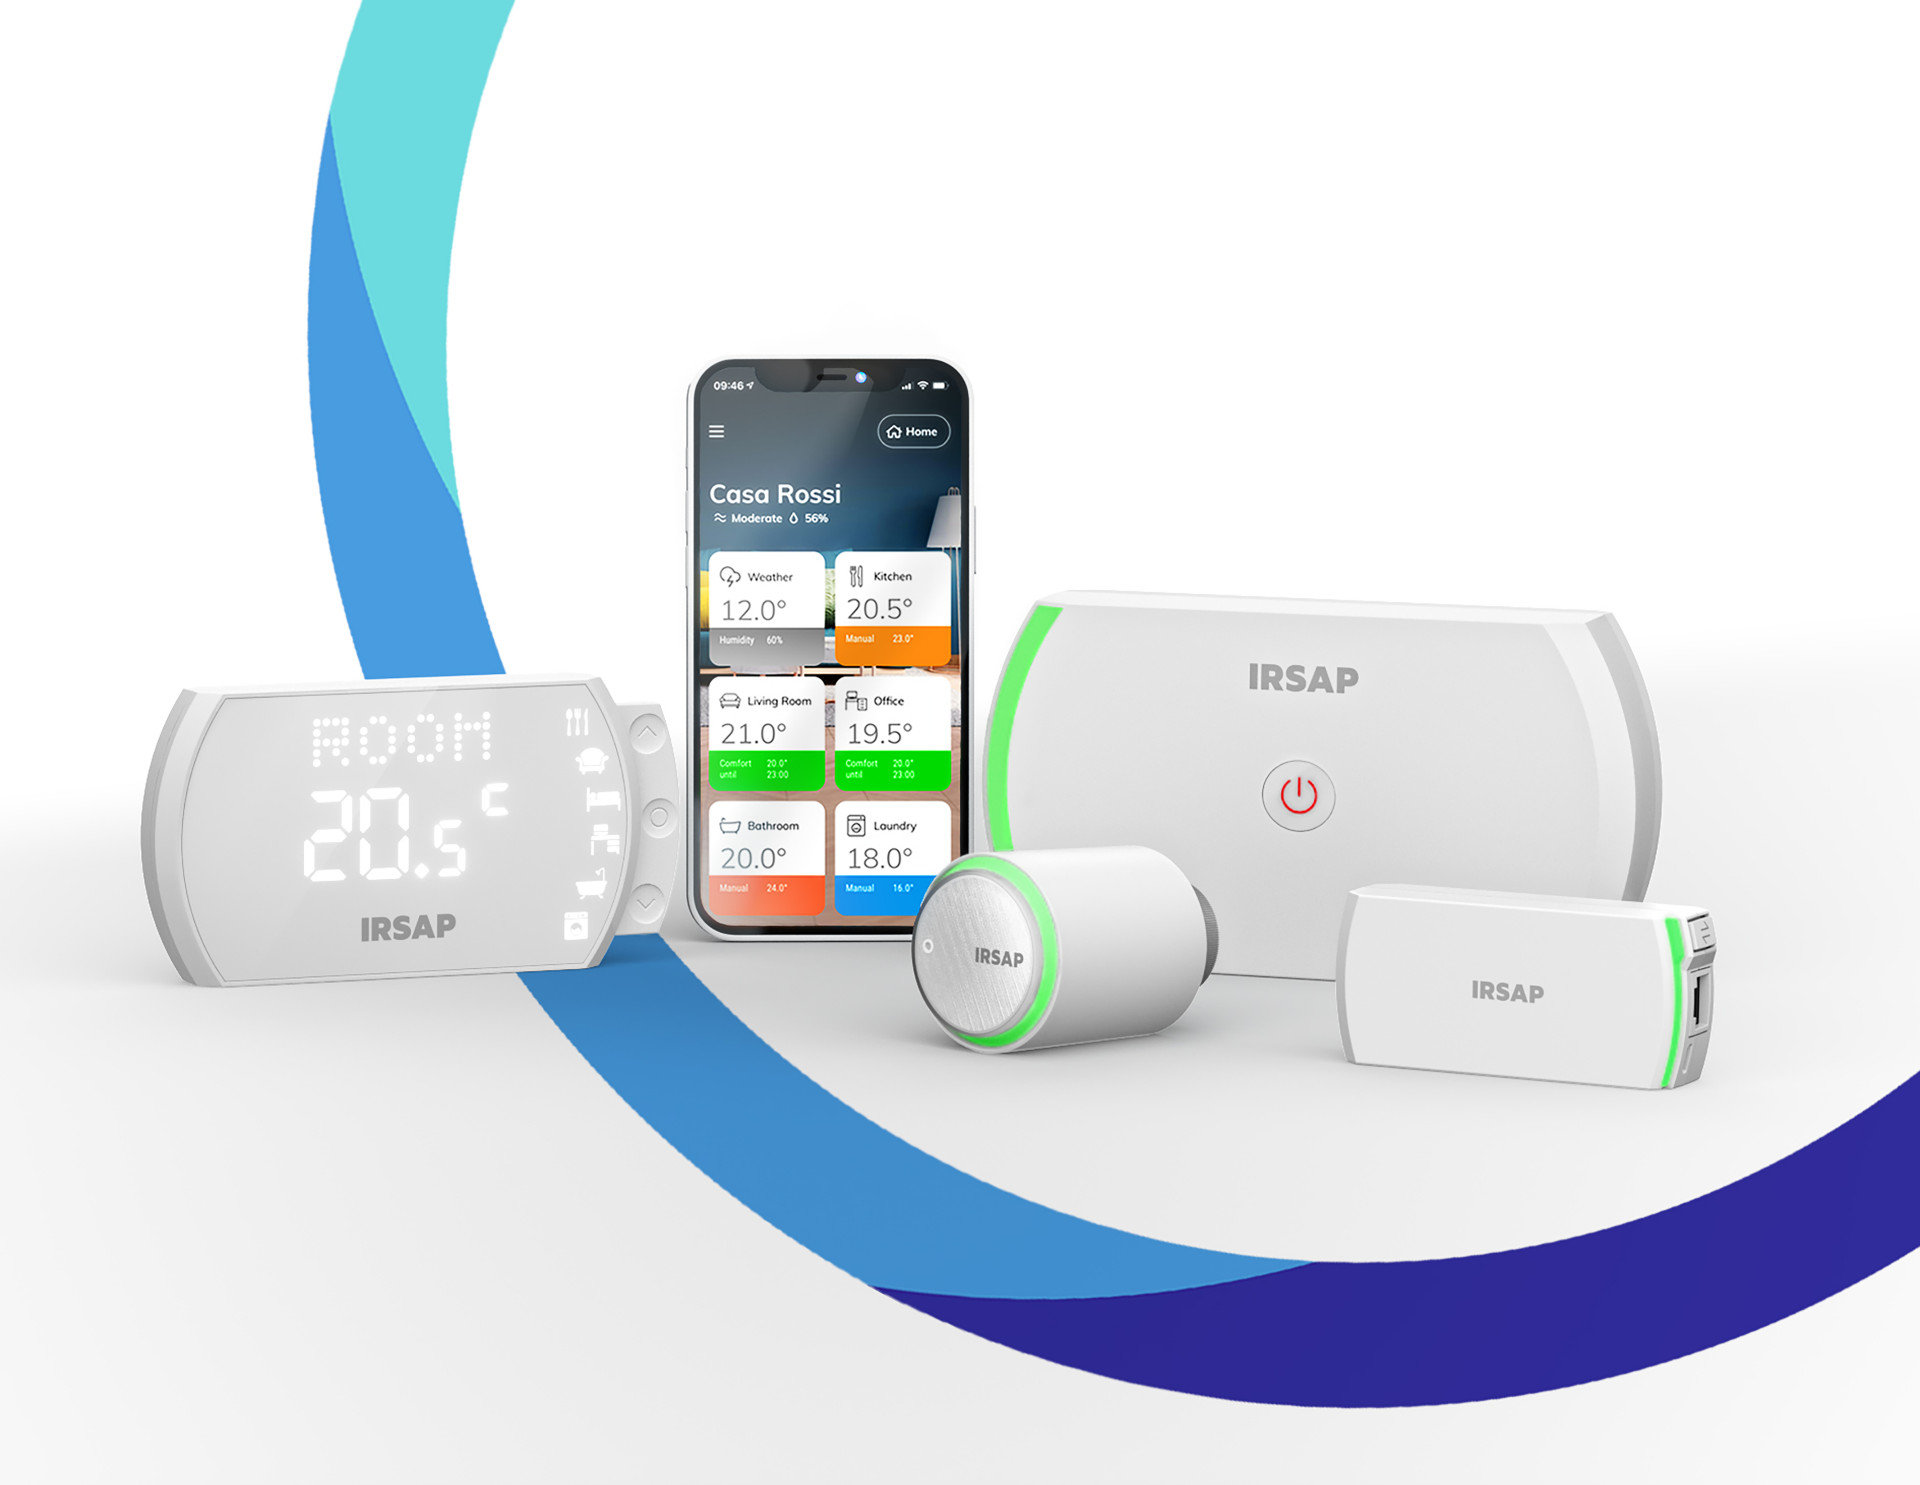
\includegraphics[width=11cm]{img/now.jpeg}
    \caption{Sistema IRSAP NOW per impianti idraulici}
    \label{fig:dispositivi_now}
\end{figure}

Una delle difficoltà attuali è l'impossibilità di andare a testare in maniera isolata i
dispositivi \Gls{rf} e l'unità centrale.

Ad esempio per validare una nuova versione \gls{firmware} della \acrshort{cu} è necessario avere a disposizione tanti dispositivi quanti
ne supporta al massimo il sistema, ovvero 48, un numero che rende molto complessa anche a
livello logistico l'operazione (si pensi ad es. solo al fatto che questi dispositivi funzionano a
batterie che dovrebbero essere continuamente mantenute cariche).

Si potrebbe quindi, mediante un'interfaccia radio opportunamente tarata sulle frequenze usate
dal sistema, andare a simulare i dispositivi lato software, consentendo con un'unica interfaccia
radio di simulare tutti i 48 dispositivi senza fisicamente averli in ufficio.

Oltre a ciò in questo progetto si può porsi anche ad un livello più basso: l'unità
centrale contiene due microcontrollori (e di conseguenza due \gls{firmware}) che comunicano fra di
loro mediante un protocollo seriale (su interfaccia \acrshort{uart}). Uno integra il ricetrasmettitore
a radiofrequenza ed è deputato a gestire la comunicazione con i dispositivi
finali, l'altro invece implementa tutte le logiche di funzionamento incluso l'interfacciamento
con il cloud, che avviene tramite porta ethernet.

Si potrebbe quindi andare a testare i due \gls{firmware} in maniera isolata l'uno dall'altro,
andando a simulare sempre tramite software la controparte mancante. Questo evita di dover
testare tutto i sistema, in particolare la parte \Gls{rf}, quando uno solo dei due software viene
aggiornato. Infatti la parte radio viene aggiornata decisamente più di rado rispetto alla
gestione delle logiche di funzionamento, ma è la più dispendiosa in termini di tempo da testare
(anche perché gestendo a livello fisico la comunicazione \Gls{rf}, in linea teorica, ogni volta andrebbero
rieseguiti i test di laboratorio per assicurarsi che i parametri radio restino nei limiti
imposti dalla normativa vigente).

\section{Test di un termostato}

In IOTINGA infine abbiamo altri progetti \gls{firmware} più complessi su cui questa metodologia
di test potrebbe essere applicata. Uno su tutti il progetto \acrfull{yat},
un cronotermostato \Gls{wifi} in grado di comunicare con la caldaia su bus \Gls{opentherm}, ma
che in futuro verrà prodotto anche in versione \Gls{modbus}.

La peculiarità di questo progetto è il fatto che è prevista l'interazione fra più
termostati mediante \Gls{ble} in modalità Long Range. In questo modo
si può gestire un impianto multizona, in cui vi è uno \acrshort{yat} \textit{master} (alimentato
dalla rete) che mantiene la connessione verso il \gls{cloud} e la comunicazione
con gli altri \acrshort{yat} \textit{slave}, che possono essere alimentati a batteria
in quanto non necessitano di una costante connessione con la rete.

Altra caratteristica dello \acrshort{yat} è un'interfaccia utente (\acrshort{hmi})
locale completa, che utilizza un display a matrice in bianco e nero (o in modelli
futuri a colori TFT) e dei pulsanti capacitivi per navigare nei vari menù. Anche
qui la sfida è riuscire a testare anche l'interfaccia utente in maniera più o meno
automatizzata. Si potrebbe ad esempio escludere completamente il display e verificare
tramite interfacciamento \Gls{spi} che il microcontrollore arrivi a scrivere i dati correttamente
nella memoria video dello schermo.

Come negli scenari visti fin ora anche qui abbiamo una possibilità di gestire configurazioni
differenti, unita al fatto che questo dispositivo verrà venduto anche in modalità ``white label'',
ossia ogni produttore potrà scegliere di andare a personalizzare alcuni aspetti e quindi
avere un \gls{firmware} differente dagli altri. Consegue quindi che ad una modifica potrebbe
corrispondere un numero elevato di binari differenti da testare, uno per cliente, e
ancora la necessità di effettuare dei test automatizzati per garantire la qualità di
quanto finisce in mano ai clienti.

\appendix

\chapter{Implementazione casi di test}
\section{Test pairing}
\label{section:impl_test_pairing}
\inputminted[]{python3}{src/test_pairing.py}

\section{Test downgrade}
\label{section:impl_test_downgrade}
\inputminted[]{python3}{src/test_downgrade.py}

\section{Test OTA}
\label{section:impl_test_ota}
\inputminted[]{python3}{src/test_ota.py}

\section{Test ripristino di fabbrica}
\label{section:impl_test_factory_reset}
\inputminted[]{python3}{src/test_factory_reset.py}

\section{Test ripristino di fabbrica disconnesso}
\label{section:impl_test_factory_reset_unbounded}
\inputminted[]{python3}{src/test_factory_reset_unbounded.py}

\section{Test termoregolazione}
\label{section:impl_test_thermoregulation}
\inputminted[]{python3}{src/test_thermoregulation.py}

\section{Test standby}
\label{section:impl_test_standby}
\inputminted[]{python3}{src/test_standby.py}

\section{Test funzionamento offline}
\label{section:impl_test_offline_working}
\inputminted[]{python3}{src/test_offline_working.py}

\clearpage

\printglossary
\printglossary[type=\acronymtype]

\end{document}
